\documentclass[11pt,a4paper]{article}
\usepackage[utf8]{inputenc}
\usepackage[T1]{fontenc}
\renewcommand{\tablename}{Tabla}
\renewcommand{\figurename}{Figura}
\renewcommand{\contentsname}{Contenido}
\renewcommand{\abstractname}{Resumen}
\renewcommand{\appendixname}{Apéndice}
\usepackage{amsmath,amssymb,amsfonts,bm}
\usepackage{graphicx}
\usepackage{booktabs}
\usepackage[a4paper,margin=2.4cm]{geometry}
\usepackage{xcolor}
\usepackage{listings}
\usepackage{caption}
\usepackage{float}
\usepackage{setspace}
\usepackage[colorlinks=true,linkcolor=blue!50!black,urlcolor=blue!50!black]{hyperref}
\graphicspath{{figuras/}}
\setstretch{1.08}
\captionsetup{font=small,labelfont=bf}

\newcommand{\vect}[1]{\bm{#1}}
\newcommand{\dd}{\mathrm{d}}
\newcommand{\Ainv}{A^{-1}}

\lstset{
  basicstyle=\ttfamily\scriptsize, keywordstyle=\color{blue!60!black}\bfseries,
  commentstyle=\color{green!40!black}, stringstyle=\color{red!50!black},
  language=Python, numbers=left, numberstyle=\tiny\color{gray}, breaklines=true,
  frame=single, framerule=.3pt, showstringspaces=false, inputencoding=utf8, extendedchars=true,
  literate={á}{{\'a}}1 {é}{{\'e}}1 {í}{{\'i}}1 {ó}{{\'o}}1 {ú}{{\'u}}1 {Á}{{\'A}}1 {ñ}{{\~n}}1
}

\title{\textbf{Física Computacional II}\\[2mm]
Taller Práctico: Soluciones Numéricas Lineales y No Lineales\\en Sistemas Físicos\\[3mm]
\large Informe técnico comparativo}
\author{Universidad de Pamplona --- Facultad de Ciencias Básicas\\Departamento de Física\\[2mm]
Estudiante: Cristian Alberto Vargas Vera }
\date{Septiembre de 2026}

\begin{document}
\maketitle
\begin{abstract}
Se resuelven cuatro problemas de la física con métodos numéricos programados desde cero en Python (sin \texttt{numpy.linalg.solve}, \texttt{scipy.optimize} ni rutinas equivalentes): (1) el perfil estacionario de temperatura en una barra con fuente interna, mediante eliminación de Gauss con pivoteo parcial, factorización LU tridiagonal (algoritmo de Thomas) e inversa de la matriz de coeficientes interpretada como función de Green discreta; (2) los modos normales de una cadena de cuatro masas acopladas, mediante rotaciones de Jacobi y método de la potencia con deflación; (3) la ecuación de Kepler, mediante relajación (punto fijo) y bisección, con análisis de convergencia en función de la excentricidad; y (4) la ecuación de estado de Van der Waals del CO$_2$ (Newton y secante) y un sistema no lineal $2\times2$ (relajación multivariable y Newton multivariable con Jacobiana). Cada resultado numérico se contrasta con una solución analítica o con una referencia independiente.
\end{abstract}

\tableofcontents
\newpage

%=====================================================================
\section{Introducción, alcance y metodología}
%=====================================================================
El taller pide aplicar métodos de álgebra lineal numérica y de resolución de ecuaciones no lineales a problemas físicos concretos. La restricción central es que cada algoritmo debe programarse a partir de su definición lógica. Por eso todo el código del informe se apoya en un único módulo, \texttt{metodos.py} (reproducido íntegro en el Apéndice~A), donde cada método es una función con bucles explícitos: \texttt{gauss\_pivoteo}, \texttt{lu\_doolittle}, \texttt{thomas\_factor}, \texttt{thomas\_resolver}, \texttt{inversa\_por\_columnas}, \texttt{jacobi\_eigen}, \texttt{potencia\_con\_deflacion}, \texttt{relajacion\_1d}, \texttt{biseccion}, \texttt{newton\_1d}, \texttt{secante}, \texttt{relajacion\_2d} y \texttt{newton\_nd}. NumPy se emplea solo como contenedor de arreglos y Matplotlib solo para graficar. Los cuatro programas \texttt{problema1.py}, \dots, \texttt{problema4.py} importan ese módulo, ejecutan los experimentos y escriben las tablas (carpeta \texttt{tablas/}) y figuras (carpeta \texttt{figuras/}) que aparecen aquí, de modo que ninguna cifra del informe fue transcrita a mano.

Un criterio se repite en los cuatro problemas: un método numérico no se da por bueno hasta compararlo con algo independiente. Cuando existe solución analítica (barra, cadena de masas, sistema $z^3=1$) se calcula el error absoluto contra ella; cuando no existe (ecuación de Kepler, Van der Waals) se toma como referencia la raíz obtenida con un método distinto y con tolerancia mucho más estricta, y se verifica además el residuo $|f(x)|$. En las gráficas de convergencia se usa la escala semilogarítmica $\log(\text{error})$ frente a la iteración, en la cual un método de convergencia lineal aparece como una recta de pendiente $\ln\rho$ y uno de convergencia cuadrática como una curva que se hunde cada vez más rápido.

Para el orden de convergencia se usa la definición estándar: un método tiene orden $p$ si $e_{k+1}\approx C\,e_k^{\,p}$ con $e_k=|x_k-x^*|$. A partir de tres errores consecutivos se estima
\begin{equation}
p_k \;=\; \frac{\ln(e_{k+1}/e_k)}{\ln(e_k/e_{k-1})}. \label{eq:orden}
\end{equation}

%=====================================================================
\section{Problema 1: perfil estacionario de temperatura en una barra 1D}
%=====================================================================
\paragraph{Deducción del sistema lineal.}
Una barra delgada de longitud $L=1.0$ m y conductividad $k=45$ W/(m\,K) tiene extremos a $T(0)=T_A=100\,^\circ$C y $T(L)=T_B=20\,^\circ$C, y una fuente volumétrica $q(x)$. En régimen estacionario, la ley de Fourier $J=-k\,\dd T/\dd x$ y la conservación de la energía $\dd J/\dd x=q$ dan la ecuación de Poisson unidimensional
\begin{equation}
-\frac{\dd^2T}{\dd x^2}=\frac{q(x)}{k}. \label{eq:poisson}
\end{equation}
Se divide $[0,L]$ en $N+1$ intervalos de ancho $\Delta x=L/(N+1)$, con nodos $x_i=i\,\Delta x$, $i=0,\dots,N+1$; los nodos $x_0=0$ y $x_{N+1}=L$ llevan la temperatura conocida y los $N$ nodos internos son las incógnitas. Los desarrollos de Taylor de $T$ alrededor de $x_i$ son
\[
T_{i\pm1}=T_i\pm\Delta x\,T'_i+\tfrac{\Delta x^2}{2}T''_i\pm\tfrac{\Delta x^3}{6}T'''_i+\tfrac{\Delta x^4}{24}T^{(4)}_i\pm\cdots
\]
y al sumar ambos se cancelan los términos impares:
\begin{equation}
\frac{T_{i-1}-2T_i+T_{i+1}}{\Delta x^2}=T''_i+\frac{\Delta x^2}{12}T^{(4)}_i+O(\Delta x^4). \label{eq:taylor}
\end{equation}
Al sustituir $T''_i=-q_i/k$ y despreciar el término de orden $\Delta x^2$ se obtiene la ecuación de diferencias del enunciado,
\begin{equation}
-T_{i-1}+2T_i-T_{i+1}=\frac{\Delta x^2}{k}\,q(x_i),\qquad i=1,\dots,N. \label{eq:difs}
\end{equation}
La ecuación~\eqref{eq:taylor} anticipa el comportamiento del error: el esquema es de segundo orden y su error local es proporcional a la cuarta derivada de la solución. Si $T^{(4)}\equiv0$ (soluciones polinómicas hasta grado 3) el esquema es exacto en los nodos, un hecho que se comprobará numéricamente.

En las ecuaciones $i=1$ e $i=N$ aparecen $T_0=T_A$ y $T_{N+1}=T_B$, que son datos y no incógnitas; por eso pasan al lado derecho. El resultado es $A\vect T=\vect b$ con
\begin{equation}
A=\begin{pmatrix}
\phantom{-}2&-1&&&&\\-1&\phantom{-}2&-1&&&\\&-1&\phantom{-}2&-1&&\\&&-1&\phantom{-}2&-1&\\&&&-1&\phantom{-}2&-1\\&&&&-1&\phantom{-}2
\end{pmatrix},\quad
b_i=\frac{\Delta x^2}{k}q(x_i)+\underbrace{T_A\,\delta_{i1}}_{\text{frontera izq.}}+\underbrace{T_B\,\delta_{iN}}_{\text{frontera der.}}. \label{eq:sistema}
\end{equation}
Para $N=6$: $\Delta x=1/7=0.142857$ m, $\Delta x^2/k=4.5351\times10^{-4}$ m$^2\cdot$K/W y nodos $x_i=i/7$. Con la fuente uniforme $q_1=5000$ W/m$^3$ resulta $\Delta x^2q_1/k=2.26757$ K y
\[
\vect b^{(1)}=(102.26757,\;2.26757,\;2.26757,\;2.26757,\;2.26757,\;22.26757)^{\!\top}.
\]

La matriz $A$ es simétrica, tridiagonal y definida positiva; sus eigenvalores son $\lambda_j=2-2\cos(j\pi/(N+1))$, todos positivos, con $\lambda_{\min}=0.198$ y $\lambda_{\max}=3.802$ para $N=6$, luego su número de condición es $\kappa_2=19.2$. Además tiene diagonal débilmente dominante y $\det A=N+1=7$ (se justificará en la factorización LU). Todo esto garantiza que el sistema tiene solución única y que los algoritmos que siguen no necesitan pivoteo para ser estables; aun así se implementa el pivoteo parcial porque es lo que pide el taller y porque es imprescindible en el caso general.

\paragraph{Eliminación de Gauss con pivoteo parcial y sustitución inversa.}
Sea $[A|\vect b]$ la matriz aumentada. En el paso $k=1,\dots,N-1$: (i) se busca la fila $p\ge k$ con mayor $|a_{pk}|$ y se intercambia con la fila $k$ (pivoteo parcial); (ii) para cada $i>k$ se calcula el multiplicador $m_{ik}=a_{ik}/a_{kk}$ y se hace $F_i\leftarrow F_i-m_{ik}F_k$, lo que anula la columna $k$ bajo la diagonal. Al terminar queda un sistema triangular superior $U\vect T=\vect c$ que se resuelve desde abajo:
\begin{equation}
T_N=\frac{c_N}{u_{NN}},\qquad T_i=\frac{1}{u_{ii}}\Big(c_i-\sum_{j=i+1}^{N}u_{ij}T_j\Big),\quad i=N-1,\dots,1. \label{eq:back}
\end{equation}
El coste es $\tfrac23N^3$ operaciones para la eliminación y $N^2$ para la sustitución.

Para $N=6$ el programa no realizó ningún intercambio de filas, como se espera de una matriz diagonalmente dominante: en cada columna la diagonal ya es el mayor elemento. Los pivotes obtenidos son $u_{ii}=2,\,\tfrac32,\,\tfrac43,\,\tfrac54,\,\tfrac65,\,\tfrac76$ y el vector transformado $\vect c$ figura en la Tabla~\ref{tab:gt}. La sustitución inversa da la solución de la última columna de esa tabla, con residuo $\|A\vect T-\vect b\|_2=2.6\times10^{-14}$.

\begin{table}[H]\centering\small
\resizebox{\textwidth}{!}{\begin{tabular}{c ccc ccc}
\toprule
$i$ & $l_i$ & $u_i$ & $u_i=(i+1)/i$ & $b^{(1)}_i$ & $c_i$ (Gauss) & $T_i^{Gauss}$\\
\midrule
1 & -- & 2.000000 & 2.000000 & 102.26757 & 102.26757 & 95.37415\\
2 & -0.500000 & 1.500000 & 1.500000 & 2.26757 & 53.40136 & 88.48073\\
3 & -0.666667 & 1.333333 & 1.333333 & 2.26757 & 37.86848 & 79.31973\\
4 & -0.750000 & 1.250000 & 1.250000 & 2.26757 & 30.66893 & 67.89116\\
5 & -0.800000 & 1.200000 & 1.200000 & 2.26757 & 26.80272 & 54.19501\\
6 & -0.833333 & 1.166667 & 1.166667 & 22.26757 & 44.60317 & 38.23129\\
\bottomrule
\end{tabular}
}
\caption{Factorización LU tridiagonal ($l_i$, $u_i$) y eliminación de Gauss ($\vect c$, $\vect T$) para $N=6$ y $q_1=5000$ W/m$^3$. Los pivotes verifican $u_i=(i+1)/i$.}\label{tab:gt}
\end{table}

Para justificar el pivoteo se resuelve el sistema $\bigl(\begin{smallmatrix}10^{-17}&1\\1&1\end{smallmatrix}\bigr)\vect x=\bigl(\begin{smallmatrix}1\\2\end{smallmatrix}\bigr)$, cuya solución exacta es $x_1\approx x_2\approx1$. Sin pivoteo el multiplicador es $10^{17}$; en la segunda fila $1-10^{17}$ y $2-10^{17}$ se redondean ambos a $-10^{17}$, se obtiene $x_2=1$ y luego $x_1=(1-1)/10^{-17}=0$, un resultado completamente erróneo. El programa devolvió $(0,\,1)$ sin pivoteo y $(1,\,1)$ con pivoteo (intercambio de las filas 1 y 2). El pivoteo evita dividir por números pequeños, que amplifican el error de redondeo.

\paragraph{Descomposición LU tridiagonal (algoritmo de Thomas).}
Si $A=LU$ y $A$ es tridiagonal (subdiagonal $a_i=-1$, diagonal $b_i=2$, superdiagonal $c_i=-1$), los factores conservan la estructura de banda: $L$ es bidiagonal inferior con diagonal unitaria y subdiagonal $l_i$, y $U$ es bidiagonal superior con diagonal $u_i$ y superdiagonal igual a la de $A$. Al igualar entradas de $LU$ con las de $A$ resulta
\begin{equation}
u_1=b_1,\qquad l_i=\frac{a_i}{u_{i-1}},\qquad u_i=b_i-l_i\,c_{i-1}\quad(i=2,\dots,N), \label{eq:thomasLU}
\end{equation}
que cuesta $O(N)$. Para esta matriz $l_i=-1/u_{i-1}$ y $u_i=2-1/u_{i-1}$, y por inducción $u_i=(i+1)/i$: es cierto para $i=1$ y si $u_{i-1}=i/(i-1)$ entonces $u_i=2-(i-1)/i=(i+1)/i$. De ahí $l_i=-(i-1)/i$ para $i=2,\dots,N$ (valores $-\tfrac12,-\tfrac23,\dots,-\tfrac56$ en la Tabla~\ref{tab:gt}) y $\det A=\prod u_i=N+1=7$. Como control se calculó también la factorización general de Doolittle (\texttt{lu\_doolittle}, coste $O(N^3)$): coincide con la de Thomas exactamente y $\|LU-A\|_{\max}=0$.

Resolver $A\vect T=\vect b$ equivale a resolver dos sistemas triangulares baratos: $L\vect y=\vect b$ (sustitución progresiva, $y_1=b_1$, $y_i=b_i-l_iy_{i-1}$) y $U\vect T=\vect y$ (sustitución regresiva, $T_N=y_N/u_N$, $T_i=(y_i-c_iT_{i+1})/u_i$), con un coste total de unas $5N$ operaciones. La ventaja decisiva es que $L$ y $U$ dependen solo de $A$, es decir de la geometría y del tipo de frontera, y no de la fuente. Así, los tres perfiles pedidos,
\[
q_1=5000,\qquad q_2=\frac{10000\,x}{L},\qquad q_3=8000\sin\frac{\pi x}{L},
\]
se resuelven con una sola factorización y tres pares de sustituciones; el programa nunca vuelve a factorizar.

Las soluciones analíticas de la ecuación~\eqref{eq:poisson} con las mismas fronteras son (se integra dos veces e imponen $T(0)=T_A$, $T(L)=T_B$):
\begin{align}
T_1(x)&=T_A+(T_B-T_A)\frac xL+\frac{5000}{2k}\,x(L-x),\\
T_2(x)&=T_A+(T_B-T_A)\frac xL+\frac{10000}{6kL}\,(L^2x-x^3),\\
T_3(x)&=T_A+(T_B-T_A)\frac xL+\frac{8000}{k}\Big(\frac L\pi\Big)^{2}\sin\frac{\pi x}{L}.
\end{align}
La Tabla~\ref{tab:T} compara ambas soluciones y la Figura~\ref{fig:perfiles} las grafica. Los resultados de Gauss y de Thomas coinciden en todas las cifras (diferencia máxima $0$ en los tres casos).

\begin{table}[H]\centering\small
\resizebox{\textwidth}{!}{\begin{tabular}{c c cc cc cc}
\toprule
 & & \multicolumn{2}{c}{$q_1$} & \multicolumn{2}{c}{$q_2$} & \multicolumn{2}{c}{$q_3$}\\
$i$ & $x_i$ [m] & Thomas & Exacta & Thomas & Exacta & Thomas & Exacta\\
\midrule
1 & 0.1429 & 95.3741 & 95.3741 & 93.7545 & 93.7545 & 96.5193 & 96.3868\\
2 & 0.2857 & 88.4807 & 88.4807 & 86.8610 & 86.8610 & 91.4645 & 91.2257\\
3 & 0.4286 & 79.3197 & 79.3197 & 78.6718 & 78.6718 & 83.5731 & 83.2753\\
4 & 0.5714 & 67.8912 & 67.8912 & 68.5390 & 68.5390 & 72.1445 & 71.8468\\
5 & 0.7143 & 54.1950 & 54.1950 & 55.8147 & 55.8147 & 57.1788 & 56.9400\\
6 & 0.8571 & 38.2313 & 38.2313 & 39.8510 & 39.8510 & 39.3765 & 39.2440\\
\bottomrule
\end{tabular}
}
\caption{Temperaturas nodales [$^\circ$C] para $N=6$: solución numérica (Thomas) frente a la solución analítica.}\label{tab:T}
\end{table}

\begin{figure}[H]\centering
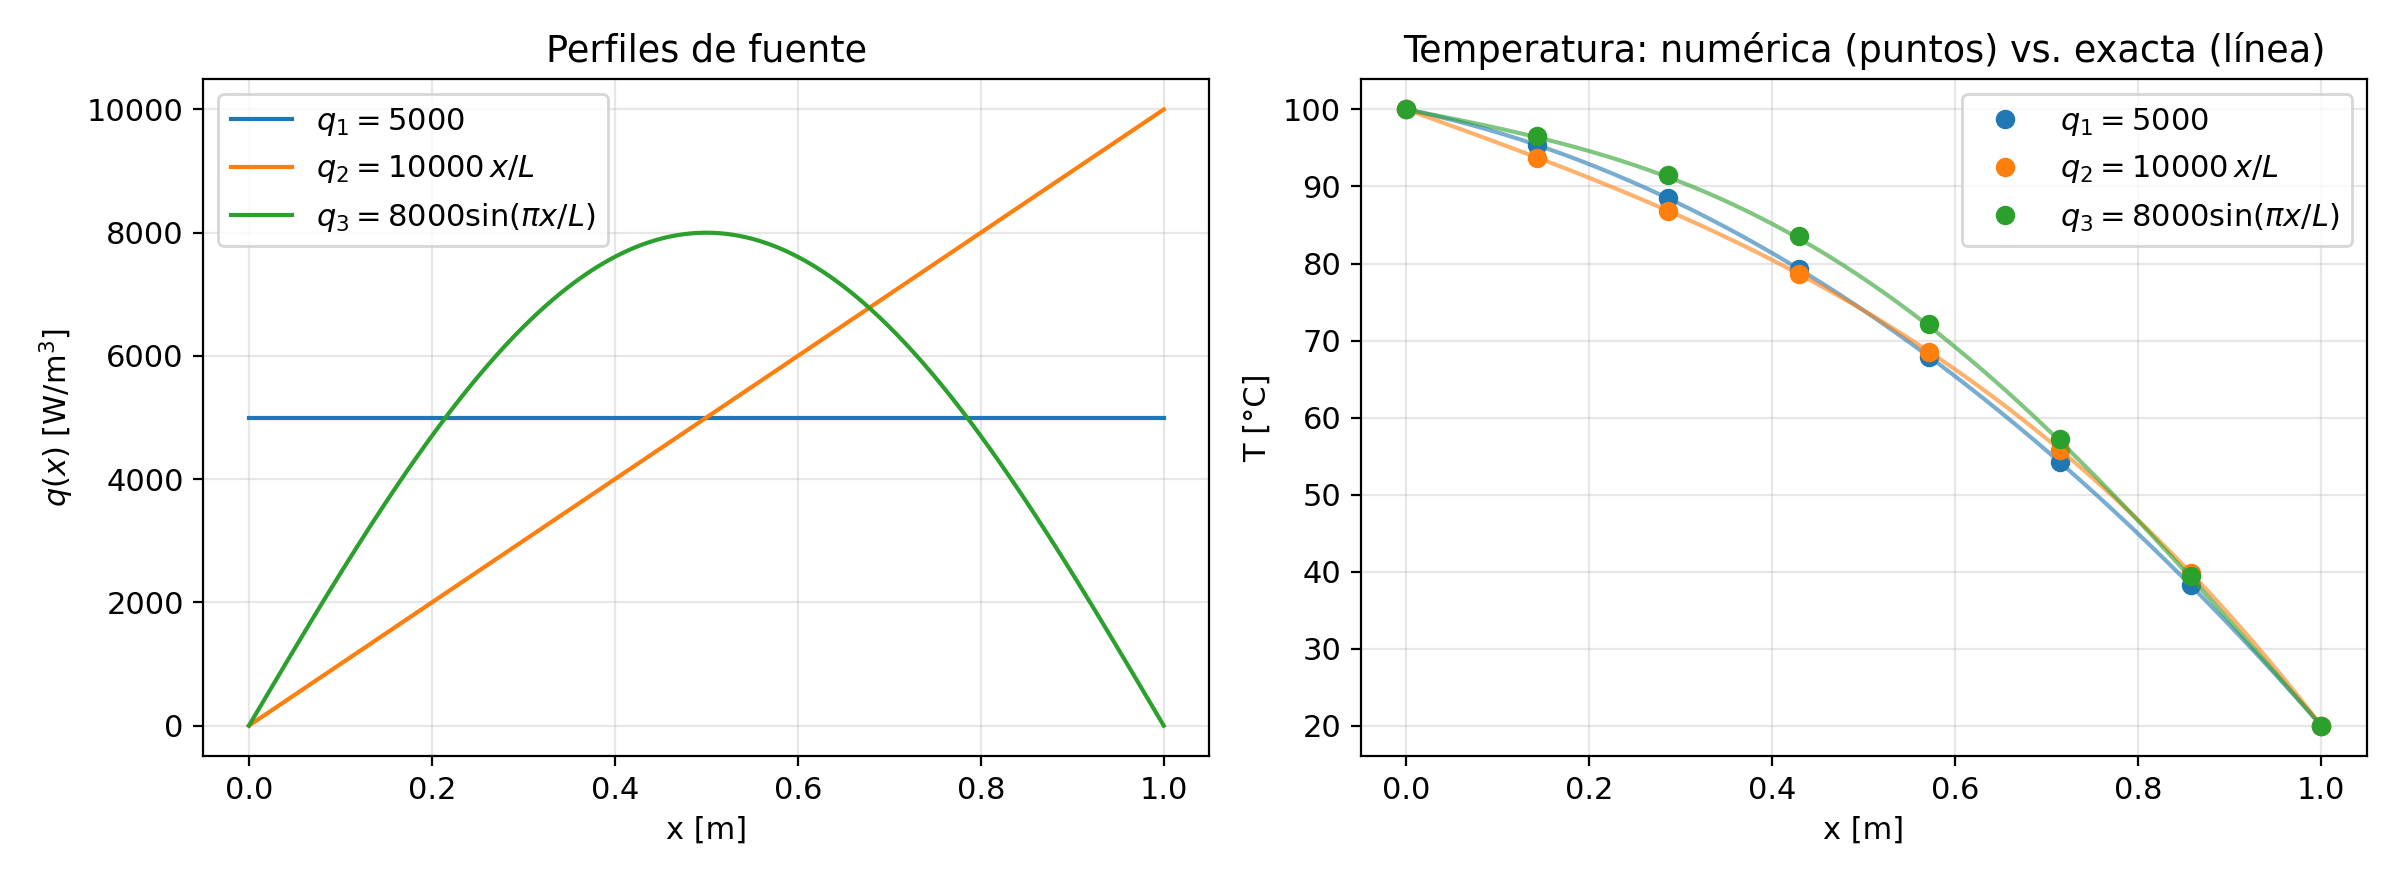
\includegraphics[width=\textwidth]{p1_perfiles.png}
\caption{Izquierda: los tres perfiles de fuente. Derecha: temperatura numérica (puntos) y analítica (líneas) para $N=6$.}\label{fig:perfiles}
\end{figure}

Los errores máximos en los nodos son $2.8\times10^{-14}$ ºC para $q_1$ y $1.4\times10^{-14}$ ºC para $q_2$ (ruido de redondeo), pero $0.298$ ºC para $q_3$. Esto confirma lo anticipado en \eqref{eq:taylor}: para $q_1$ la solución es un polinomio de grado 2 y para $q_2$ de grado 3, así que $T^{(4)}=0$ y el esquema es exacto en los nodos. Para $q_3$ la solución contiene un seno cuya cuarta derivada no se anula, con $T_3^{(4)}=(8000/k)(\pi/L)^2\sin(\pi x/L)$ y valor máximo $1755$ K/m$^4$. El error $\varepsilon$ del esquema satisface aproximadamente $-\varepsilon''=\tfrac{\Delta x^2}{12}T^{(4)}$, cuya solución en el centro es $\tfrac{\Delta x^2}{12}(L/\pi)^2\,1755=0.302$ ºC, muy cercana al valor observado $0.298$ ºC. La Tabla~\ref{tab:malla} muestra que, al refinar la malla, el error decae con orden $1.98\to2.00$, como corresponde a un esquema de segundo orden.

\begin{table}[H]\centering\small
\begin{tabular}{r c c}
\toprule
$N$ & $\max_i|T_i-T(x_i)|$ & orden observado\\
\midrule
6 & 2.978e-01 & --\\
12 & 8.728e-02 & 1.98\\
25 & 2.193e-02 & 1.99\\
50 & 5.694e-03 & 2.00\\
100 & 1.452e-03 & 2.00\\
200 & 3.667e-04 & 2.00\\
400 & 9.213e-05 & 2.00\\
\bottomrule
\end{tabular}

\caption{Error máximo nodal para el perfil $q_3$ en función del número de nodos, y orden de convergencia observado.}\label{tab:malla}
\end{table}

Una comprobación física independiente es el balance de energía para $q_1$: el flujo de calor $J=-k\,T'$ vale $J(0)=+1100$ W/m$^2$ y $J(L)=+6100$ W/m$^2$, y su diferencia $5000$ W/m$^2$ es exactamente lo que genera la fuente en la barra ($q_1L$ por unidad de área). El extremo frío evacua entonces el calor entrante por el extremo caliente más el generado internamente. El perfil resultante es monótono decreciente: la fuente eleva la temperatura por encima de la recta que une las fronteras, pero no lo suficiente para crear un máximo interior.

\begin{figure}[H]\centering
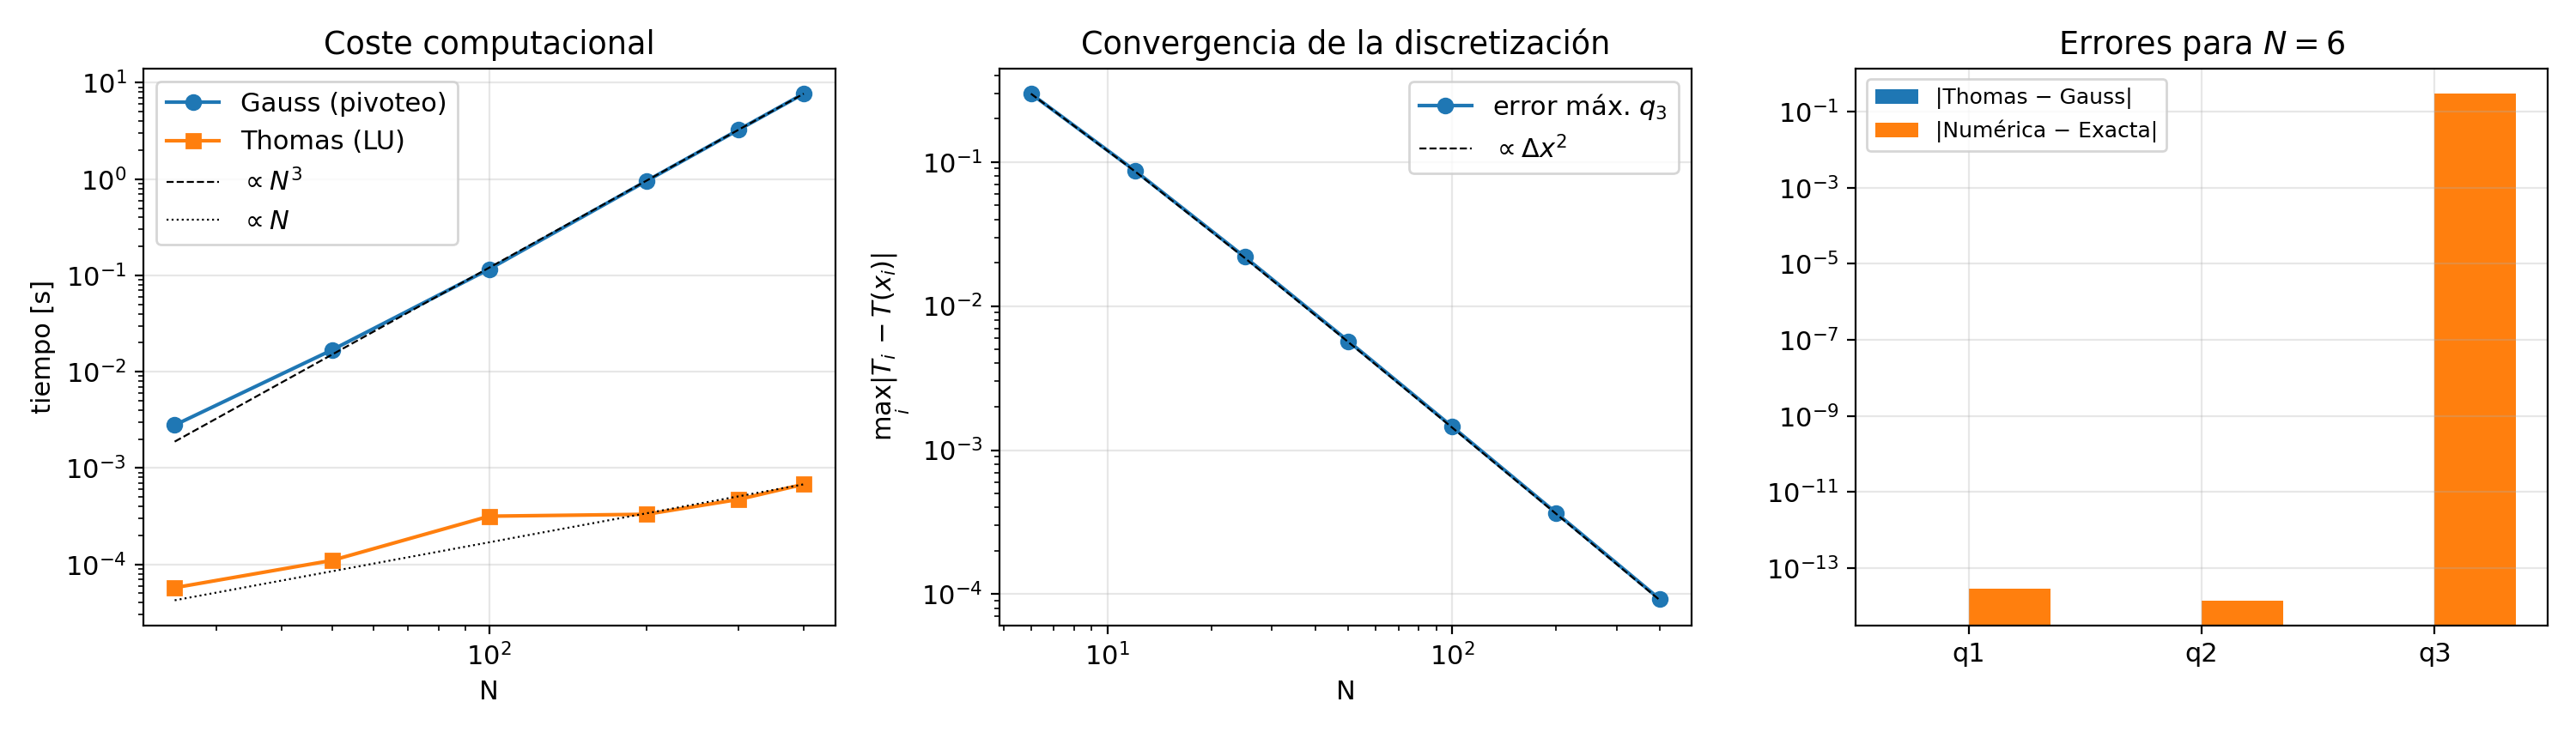
\includegraphics[width=\textwidth]{p1_coste_error.png}
\caption{Izquierda: tiempo de cálculo frente a $N$ (Gauss crece como $N^3$, Thomas como $N$). Centro: convergencia de la discretización para $q_3$. Derecha: errores para $N=6$ (escala logarítmica).}\label{fig:coste}
\end{figure}

\begin{table}[H]\centering\small
\begin{tabular}{r cc c}
\toprule
$N$ & $t_{Gauss}$ [ms] & $t_{Thomas}$ [ms] & $t_G/t_T$\\
\midrule
25 & 2.79 & 0.057 & 49\\
50 & 16.82 & 0.110 & 153\\
100 & 116.33 & 0.317 & 367\\
200 & 955.38 & 0.331 & 2884\\
300 & 3247.02 & 0.472 & 6875\\
400 & 7707.61 & 0.678 & 11363\\
\bottomrule
\end{tabular}

\caption{Tiempos medidos (Python puro, un solo sistema $q_3$).}\label{tab:coste}
\end{table}

La Figura~\ref{fig:coste} y la Tabla~\ref{tab:coste} cuantifican el argumento sobre el coste. Con $N=400$ nodos, Gauss (Python puro, bucles explícitos) tarda del orden de segundos frente a fracciones de milisegundo de Thomas, y la razón crece con $N^2$. Esto es lo que hace viable resolver Poisson en mallas finas, o repetirlo para muchas fuentes.

\paragraph{Inversa de $A$ y función de Green discreta.}
La inversa se obtiene resolviendo $A\vect x_j=\vect e_j$ para $j=1,\dots,N$, con $\vect e_j$ la columna $j$ de la identidad; las columnas $\vect x_j$ forman $\Ainv=[\vect x_1\,|\cdots|\,\vect x_N]$. Cada sistema reutiliza $L$ y $U$, de modo que las $N$ soluciones cuestan $O(N^2)$ en total. El resultado es
\[
7\,A^{-1}=\begin{pmatrix}
6 & 5 & 4 & 3 & 2 & 1\\
5 & 10 & 8 & 6 & 4 & 2\\
4 & 8 & 12 & 9 & 6 & 3\\
3 & 6 & 9 & 12 & 8 & 4\\
2 & 4 & 6 & 8 & 10 & 5\\
1 & 2 & 3 & 4 & 5 & 6\\
\end{pmatrix}
\]

con $\|A\Ainv-I\|_{\max}=2.2\times10^{-16}$; el cálculo con Gauss da una matriz idéntica y $\|\Ainv\vect b-\vect T\|_{\max}=1.4\times10^{-14}$. La estructura sugiere una fórmula cerrada,
\begin{equation}
(\Ainv)_{ij}=\frac{\min(i,j)\,\big(N+1-\max(i,j)\big)}{N+1}, \label{eq:green}
\end{equation}
que el programa verifica con error $4\times10^{-16}$. Se demuestra directamente: para $i\ne j$ la columna $j$ es lineal en $i$ a cada lado de $j$, luego su segunda diferencia es nula; en $i=j$ la pendiente pasa de $(N+1-j)/(N+1)$ a $-j/(N+1)$ y por tanto $-G_{j-1,j}+2G_{jj}-G_{j+1,j}=\frac{(N+1-j)+j}{N+1}=1$. Así $A\Ainv=I$.

La interpretación física es la siguiente. Como $\vect T=\Ainv\vect b$, la entrada $(\Ainv)_{ij}$ es la temperatura que aparece en el nodo $i$ por cada unidad de término independiente en el nodo $j$, es decir, la respuesta del sistema a una fuente puntual unitaria. Separando el aporte de las fronteras y el de la fuente,
\begin{equation}
T_i=\underbrace{T_A\Big(1-\frac{x_i}{L}\Big)+T_B\frac{x_i}{L}}_{\Ainv(T_A\vect e_1+T_B\vect e_N)}+\sum_{j=1}^N(\Ainv)_{ij}\,\frac{\Delta x^2}{k}q_j
=T^{\rm lin}(x_i)+\sum_{j=1}^N G(x_i,x_j)\,\frac{q_j}{k}\,\Delta x, \label{eq:superp}
\end{equation}
donde $G(x,x')=\Delta x\,(\Ainv)_{ij}=x_<(L-x_>)/L$, con $x_<=\min(x,x')$ y $x_>=\max(x,x')$, es la función de Green continua del operador $-\dd^2/\dd x^2$ con condiciones nulas en los bordes; la suma en~\eqref{eq:superp} es la suma de Riemann de $\int_0^LG(x,x')\,q(x')/k\,\dd x'$. Por eso la matriz inversa es la versión discreta de la función de Green y resume el principio de superposición del problema lineal: cualquier fuente es una combinación de fuentes puntuales, y la respuesta es la combinación correspondiente de las columnas de $\Ainv$. Otras propiedades se leen en la matriz (Figura~\ref{fig:inversa}): es simétrica, $G_{ij}=G_{ji}$ (reciprocidad: la respuesta en $i$ a una fuente en $j$ es igual a la respuesta en $j$ a una fuente en $i$); es positiva, pues una fuente de calor nunca enfría ningún punto; su máximo está en el centro de la barra (el valor $12/7=1.71$ K por unidad de fuente, en los nodos 3 y 4), lo más alejado de ambos sumideros a temperatura fija; y cada columna es una función lineal a trozos con un pico en el nodo fuente. Como comprobación, la suma de la fila $i$ es la respuesta a una fuente uniforme y vale $i(N+1-i)/2$ (para $i=3$: $(4+8+12+9+6+3)/7=6$), que multiplicada por $\Delta x^2q/k$ reproduce el término $x(L-x)q/(2k)$ de $T_1(x)$.

\begin{figure}[H]\centering
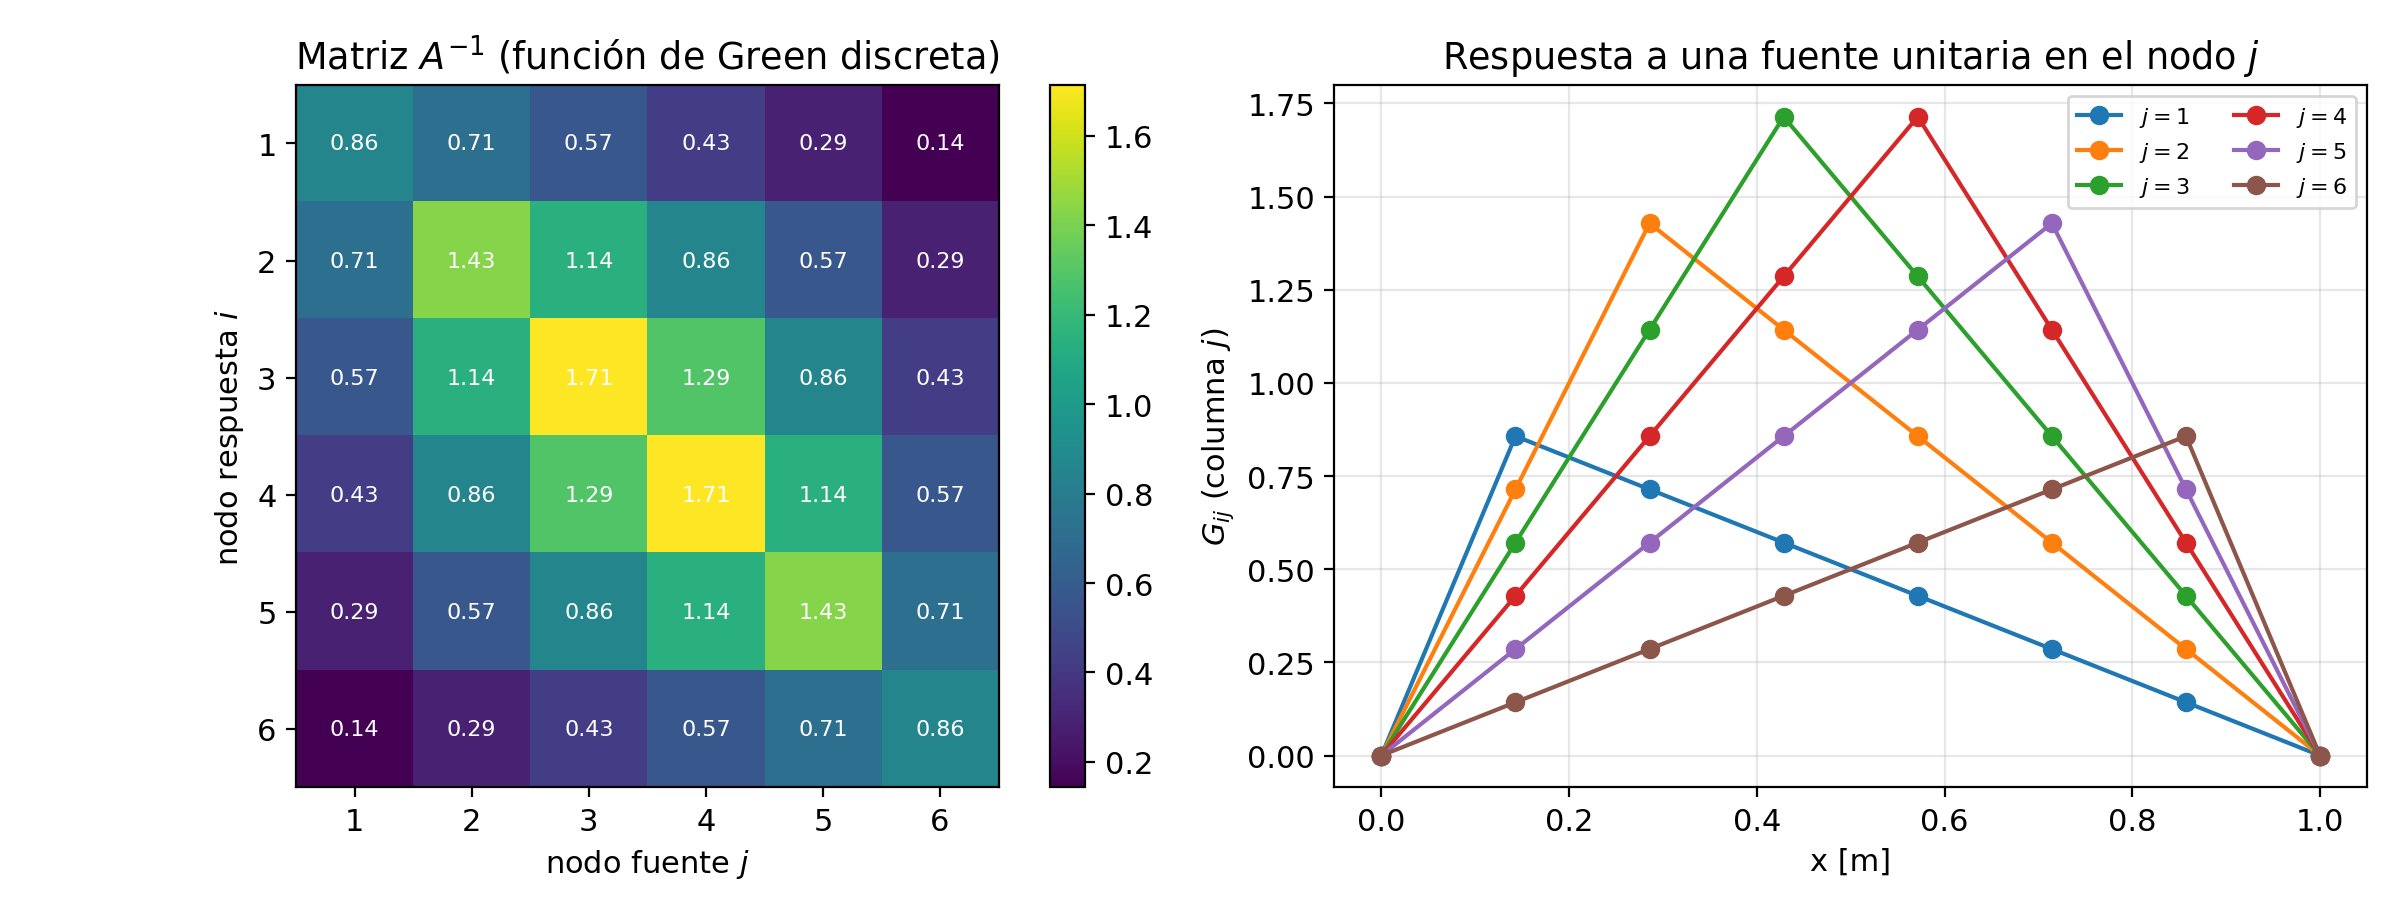
\includegraphics[width=\textwidth]{p1_inversa.png}
\caption{Izquierda: $\Ainv$ para $N=6$. Derecha: cada columna es la respuesta de la barra a una fuente puntual unitaria en el nodo $j$ (función de Green discreta).}\label{fig:inversa}
\end{figure}

%=====================================================================
\section{Problema 2: modos normales de vibración en cadenas acopladas}
%=====================================================================
\paragraph{Planteamiento y problema de eigenvalores.}
Cuatro masas iguales $m=0.5$ kg están alineadas entre dos paredes fijas y unidas por cinco resortes idénticos de constante $k=200$ N/m. Si $x_i$ es el desplazamiento longitudinal de la masa $i$ y $x_0=x_5=0$ (paredes), la segunda ley de Newton da
\[
m\ddot x_i=-k(x_i-x_{i-1})-k(x_i-x_{i+1})=k\,(x_{i-1}-2x_i+x_{i+1}),\qquad i=1,\dots,4,
\]
o, en forma matricial, $M\ddot{\vect x}=-K\vect x$ con
\[
M=m\,I=0.5\,I,\qquad K=k\begin{pmatrix}\phantom{-}2&-1&0&0\\-1&\phantom{-}2&-1&0\\0&-1&\phantom{-}2&-1\\0&0&-1&\phantom{-}2\end{pmatrix}.
\]
Se buscan soluciones en las que todas las masas oscilan con la misma frecuencia y fase, $\vect x(t)=\vect v\cos(\omega t+\phi)$. Sustituyendo, $K\vect v=\omega^2M\vect v$, y multiplicando por $M^{-1}$,
\begin{equation}
(A-\lambda I)\vect v=0,\qquad A=M^{-1}K=\frac km\begin{pmatrix}\phantom{-}2&-1&&\\-1&\phantom{-}2&-1&\\&-1&\phantom{-}2&-1\\&&-1&\phantom{-}2\end{pmatrix}=\begin{pmatrix}\phantom{-}800&-400&0&0\\-400&\phantom{-}800&-400&0\\0&-400&\phantom{-}800&-400\\0&0&-400&\phantom{-}800\end{pmatrix}\ \mathrm{s^{-2}}, \label{eq:A}
\end{equation}
con $\lambda=\omega^2$ y $k/m=400$ s$^{-2}$ (la matriz $A$ calculada con el producto $M^{-1}K$ en el programa coincide con esta). Como $M=mI$, $A$ es simétrica; en un caso con masas distintas $M^{-1}K$ ya no lo sería y se trabajaría con $M^{-1/2}KM^{-1/2}$, que sí lo es. Al ser $K$ definida positiva (la energía potencial $\tfrac12\vect x^\top K\vect x$ es positiva para todo desplazamiento no nulo), todos los $\lambda_j$ son reales y positivos y los eigenvectores son mutuamente ortogonales, de modo que los modos son oscilaciones independientes y cualquier movimiento es su superposición.

\paragraph{Método de Jacobi (rotaciones).}
Para una matriz simétrica $A$, el método de Jacobi la lleva a forma diagonal mediante rotaciones planas sucesivas. Una rotación $P_{pq}$ (con $P_{pp}=P_{qq}=c$, $P_{pq}=s$, $P_{qp}=-s$, $c=\cos\theta$, $s=\sin\theta$) transforma $A\to A'=P^\top AP$ y modifica solo las filas y columnas $p$ y $q$. La entrada fuera de la diagonal cambia según
\[
a'_{pq}=(c^2-s^2)\,a_{pq}+sc\,(a_{pp}-a_{qq}),
\]
que se anula si $\cot2\theta=\vartheta\equiv(a_{qq}-a_{pp})/(2a_{pq})$. Con $t=\tan\theta$ esto equivale a $t^2+2\vartheta t-1=0$, y se elige la raíz de menor módulo (rotación pequeña, más estable):
\begin{equation}
t=\frac{\operatorname{sgn}\vartheta}{|\vartheta|+\sqrt{\vartheta^2+1}},\qquad c=\frac1{\sqrt{t^2+1}},\qquad s=tc. \label{eq:jacobi}
\end{equation}
Las actualizaciones son $a'_{pp}=a_{pp}-t\,a_{pq}$, $a'_{qq}=a_{qq}+t\,a_{pq}$, $a'_{rp}=c\,a_{rp}-s\,a_{rq}$ y $a'_{rq}=c\,a_{rq}+s\,a_{rp}$ para $r\ne p,q$. Como la rotación conserva la norma de Frobenius, y la diagonal aumenta lo que disminuye la parte fuera de la diagonal, cada rotación reduce la suma de cuadrados de los elementos fuera de la diagonal en exactamente $2a_{pq}^2$, así que el proceso converge. Las rotaciones se acumulan en $V\leftarrow VP$; cuando $A$ es (numéricamente) diagonal, la diagonal contiene los eigenvalores y las columnas de $V$ los eigenvectores, ortonormales por ser producto de rotaciones. El algoritmo recorre cíclicamente todos los pares $(p,q)$ en «barridos» hasta que la norma fuera de la diagonal sea menor que $10^{-13}$.

La Tabla~\ref{tab:jh} muestra la convergencia: cuatro barridos bastan, y el último es un salto de $3.4\times10^{-5}$ a $6\times10^{-17}$, característico de la convergencia cuadrática asintótica de Jacobi (Figura~\ref{fig:p2conv}, izquierda).

\begin{table}[H]\centering\small
\begin{tabular}{c c}
\toprule
 Barrido & $\lVert A_{\text{fuera de la diagonal}}\rVert_F$\\
\midrule
0 & 9.798e+02\\
1 & 2.637e+02\\
2 & 3.354e+01\\
3 & 3.353e-05\\
4 & 5.908e-17\\
\bottomrule
\end{tabular}

\caption{Norma de Frobenius de la parte fuera de la diagonal tras cada barrido de Jacobi.}\label{tab:jh}
\end{table}

\paragraph{Resultados: frecuencias naturales y eigenvectores.}
Los eigenvalores, con $\omega_j=\sqrt{\lambda_j}$, $f_j=\omega_j/2\pi$ y $T_j=1/f_j$, están en la Tabla~\ref{tab:modos}, y los eigenvectores normalizados ($\|\vect v_j\|_2=1$, primera componente positiva) en la Tabla~\ref{tab:vec}.

\begin{table}[H]\centering\small
\resizebox{\textwidth}{!}{\begin{tabular}{c ccc cc c}
\toprule
Modo & $\lambda_j$ [s$^{-2}$] (Jacobi) & $\lambda_j$ analítico & error abs. & $\omega_j$ [rad/s] & $f_j$ [Hz] & $T_j$ [ms]\\
\midrule
1 & 152.786405 & 152.786405 & 2.8e-14 & 12.36068 & 1.9673 & 508.320\\
2 & 552.786405 & 552.786405 & 2.3e-13 & 23.51141 & 3.7420 & 267.240\\
3 & 1047.213595 & 1047.213595 & 0.0e+00 & 32.36068 & 5.1504 & 194.161\\
4 & 1447.213595 & 1447.213595 & 2.3e-13 & 38.04226 & 6.0546 & 165.163\\
\bottomrule
\end{tabular}
}
\caption{Eigenvalores y frecuencias naturales de la cadena de cuatro masas (Jacobi), comparados con la fórmula analítica.}\label{tab:modos}
\end{table}
\begin{table}[H]\centering\small
\begin{tabular}{c cccc}
\toprule
 Modo & $v_{j,1}$ & $v_{j,2}$ & $v_{j,3}$ & $v_{j,4}$\\
\midrule
1 & +0.371748 & +0.601501 & +0.601501 & +0.371748\\
2 & +0.601501 & +0.371748 & -0.371748 & -0.601501\\
3 & +0.601501 & -0.371748 & -0.371748 & +0.601501\\
4 & +0.371748 & -0.601501 & +0.601501 & -0.371748\\
\bottomrule
\end{tabular}

\caption{Eigenvectores normalizados del método de Jacobi ($v_{j,i}$: componente de la masa $i$ en el modo $j$).}\label{tab:vec}
\end{table}

El problema tiene solución analítica que sirve de referencia. Se prueba $v_i=\sin(iq)$ con $q=j\pi/(N+1)$, que anula ambos extremos ($v_0=v_{N+1}=0$). Como $\sin((i-1)q)+\sin((i+1)q)=2\cos q\,\sin(iq)$,
\[
-v_{i-1}+2v_i-v_{i+1}=(2-2\cos q)\,v_i=4\sin^2\!\frac q2\,v_i,
\]
y por tanto
\begin{equation}
\lambda_j=\frac{4k}{m}\sin^2\!\frac{j\pi}{2(N+1)},\quad \omega_j=2\sqrt{\tfrac km}\,\sin\frac{j\pi}{2(N+1)}=40\sin\frac{j\pi}{10}\ \mathrm{rad/s},\quad v_{j,i}=\sqrt{\tfrac2{N+1}}\sin\frac{ij\pi}{N+1}. \label{eq:analitico}
\end{equation}
Los valores de \eqref{eq:analitico} coinciden con los del algoritmo con diferencia máxima de $2.3\times10^{-13}$ en los eigenvalores; los productos escalares $|\langle\vect v_j^{\rm Jacobi},\vect v_j^{\rm anal}\rangle|$ valen $1$ hasta $2\times10^{-16}$, los residuos $\|A\vect v_j-\lambda_j\vect v_j\|_2$ son $\lesssim3\times10^{-13}$ y $\max|V^\top V-I|=4\times10^{-16}$ (ortonormalidad). Además $\omega_1=40\sin18^\circ=12.36$ rad/s y las frecuencias satisfacen la relación de dispersión $\omega=2\omega_0\sin(qa/2)$ de una cadena discreta, con $\omega_0=\sqrt{k/m}=20$ rad/s. Existe una frecuencia de corte $2\omega_0=40$ rad/s, y el modo 4 ($38.04$ rad/s) se le acerca cuando la longitud de onda es del orden de dos espaciados.

\paragraph{Método de la potencia con deflación.}
Como método alternativo se implementó la potencia con deflación. Si $\vect x_0=\sum_ja_j\vect v_j$ con $a_1\ne0$ y $|\lambda_1|>|\lambda_2|\ge\cdots$, entonces
\[
A^n\vect x_0=\lambda_1^n\Big[a_1\vect v_1+\sum_{j\ge2}a_j\Big(\frac{\lambda_j}{\lambda_1}\Big)^{\!n}\vect v_j\Big]\;\longrightarrow\;\lambda_1^na_1\vect v_1,
\]
así que la iteración normalizada $\vect x_{n+1}=A\vect x_n/\|A\vect x_n\|$ converge al eigenvector dominante con razón $|\lambda_2/\lambda_1|$, y el cociente de Rayleigh $\lambda\approx\vect x^\top A\vect x$ (con $\|\vect x\|=1$) da el eigenvalor con error cuadrático en el error del vector, por ser $A$ simétrica. Una vez conocido $(\lambda_1,\vect v_1)$ se elimina de la matriz mediante la deflación de Hotelling,
\[
A_{(2)}=A-\lambda_1\vect v_1\vect v_1^\top,
\]
que conserva los demás pares propios (porque $\vect v_j^\top\vect v_1=0$) y anula el primero. Repitiendo se obtienen los cuatro, de mayor a menor. Las razones de convergencia teóricas son $\lambda_2/\lambda_1=0.7236$, luego $0.5279$ y $0.2764$ para los pasos siguientes, y $0$ en el último paso (solo queda un eigenvalor no nulo). Esto explica los números de iteraciones observados, $48$, $26$, $15$ y $3$ (Tabla~\ref{tab:pot} y Figura~\ref{fig:p2conv}, centro).

\begin{table}[H]\centering\small
\begin{tabular}{c c c c c}
\toprule
 Paso & $\lambda$ (potencia) & $\lambda$ (Jacobi) & iteraciones & $|\Delta\lambda|$\\
\midrule
1 & 1447.21359550 & 1447.21359550 & 48 & 9.7e-11\\
2 & 1047.21359550 & 1047.21359550 & 26 & 5.4e-11\\
3 & 552.78640450 & 552.78640450 & 15 & 7.8e-12\\
4 & 152.78640450 & 152.78640450 & 3 & 5.7e-14\\
\bottomrule
\end{tabular}

\caption{Potencia con deflación frente a Jacobi (tolerancia relativa $10^{-13}$).}\label{tab:pot}
\end{table}

Ambos métodos coinciden a $\sim10^{-10}$ en los eigenvalores y a $10^{-13}$ en el solapamiento de los eigenvectores. La diferencia mayor de la potencia se debe a que cada deflación arrastra el error del par anterior, mientras que Jacobi trabaja siempre con la matriz completa. Jacobi calcula los cuatro pares a la vez y es más preciso, mientras que la potencia es más sencilla y barata por iteración ($O(N^2)$) y es preferible cuando solo interesan los eigenvalores extremos de matrices grandes y dispersas.

\begin{figure}[H]\centering
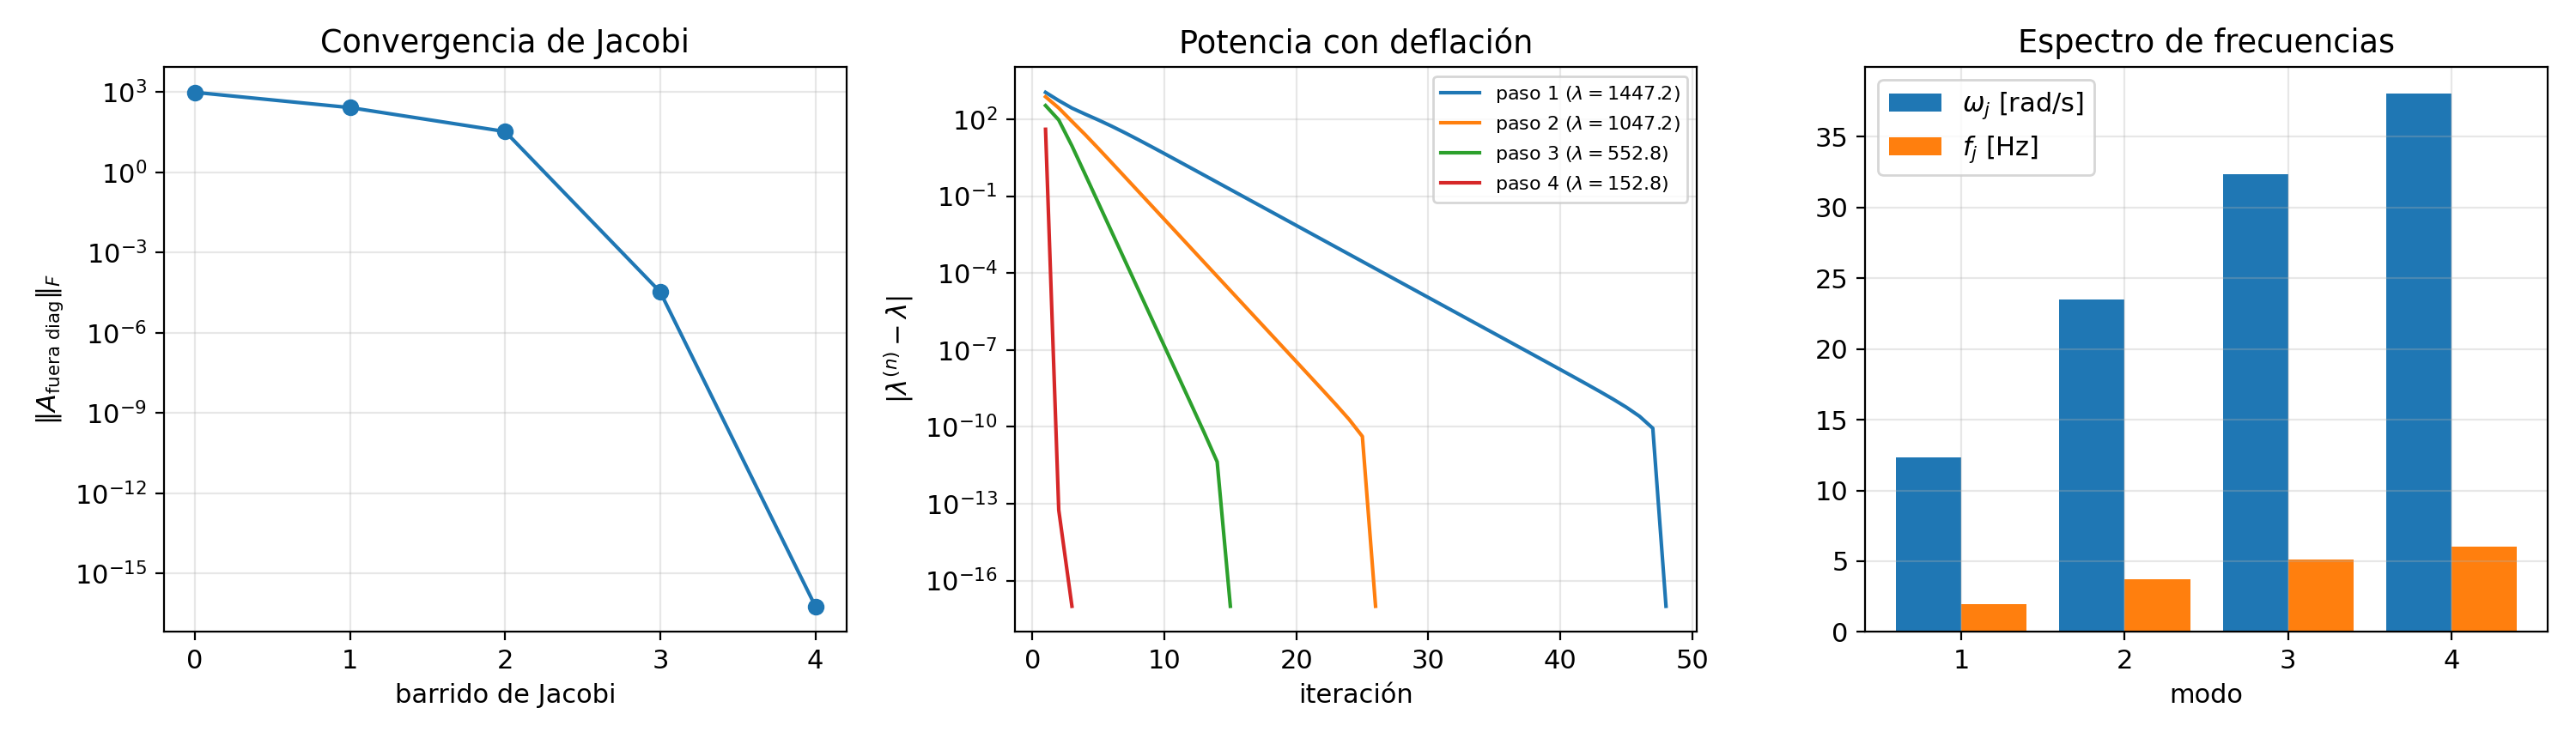
\includegraphics[width=\textwidth]{p2_convergencia.png}
\caption{Izquierda: convergencia de Jacobi. Centro: error del eigenvalor en la potencia con deflación (semilog). Derecha: espectro de frecuencias.}\label{fig:p2conv}
\end{figure}

\paragraph{Perfiles espaciales de los modos normales.}
La Figura~\ref{fig:modos} muestra los cuatro modos (puntos: eigenvectores calculados; línea punteada: onda estacionaria continua $\sin(j\pi x/5)$; las paredes se dibujan como cuadrados negros en $x=0$ y $x=5$). El modo $j$ tiene $j-1$ nodos (cambios de signo) y una simetría definida respecto del centro de la cadena: los modos 1 y 3 son simétricos (pares) y los modos 2 y 4 antisimétricos (impares), una consecuencia de la simetría de espejo de $K$. En el modo 1 todas las masas se mueven en fase (oscilación de baja frecuencia, los resortes se estiran poco); en el modo 4 masas vecinas se mueven en oposición de fase y los resortes se deforman al máximo, lo que da la frecuencia más alta. Las amplitudes en las masas coinciden con el muestreo de la onda continua, y esa es la razón de que los cuatro eigenvectores tengan solo dos valores absolutos distintos, $0.3717$ y $0.6015$ (que son $\sqrt{2/5}\sin36^\circ$ y $\sqrt{2/5}\sin72^\circ$).

\begin{figure}[H]\centering
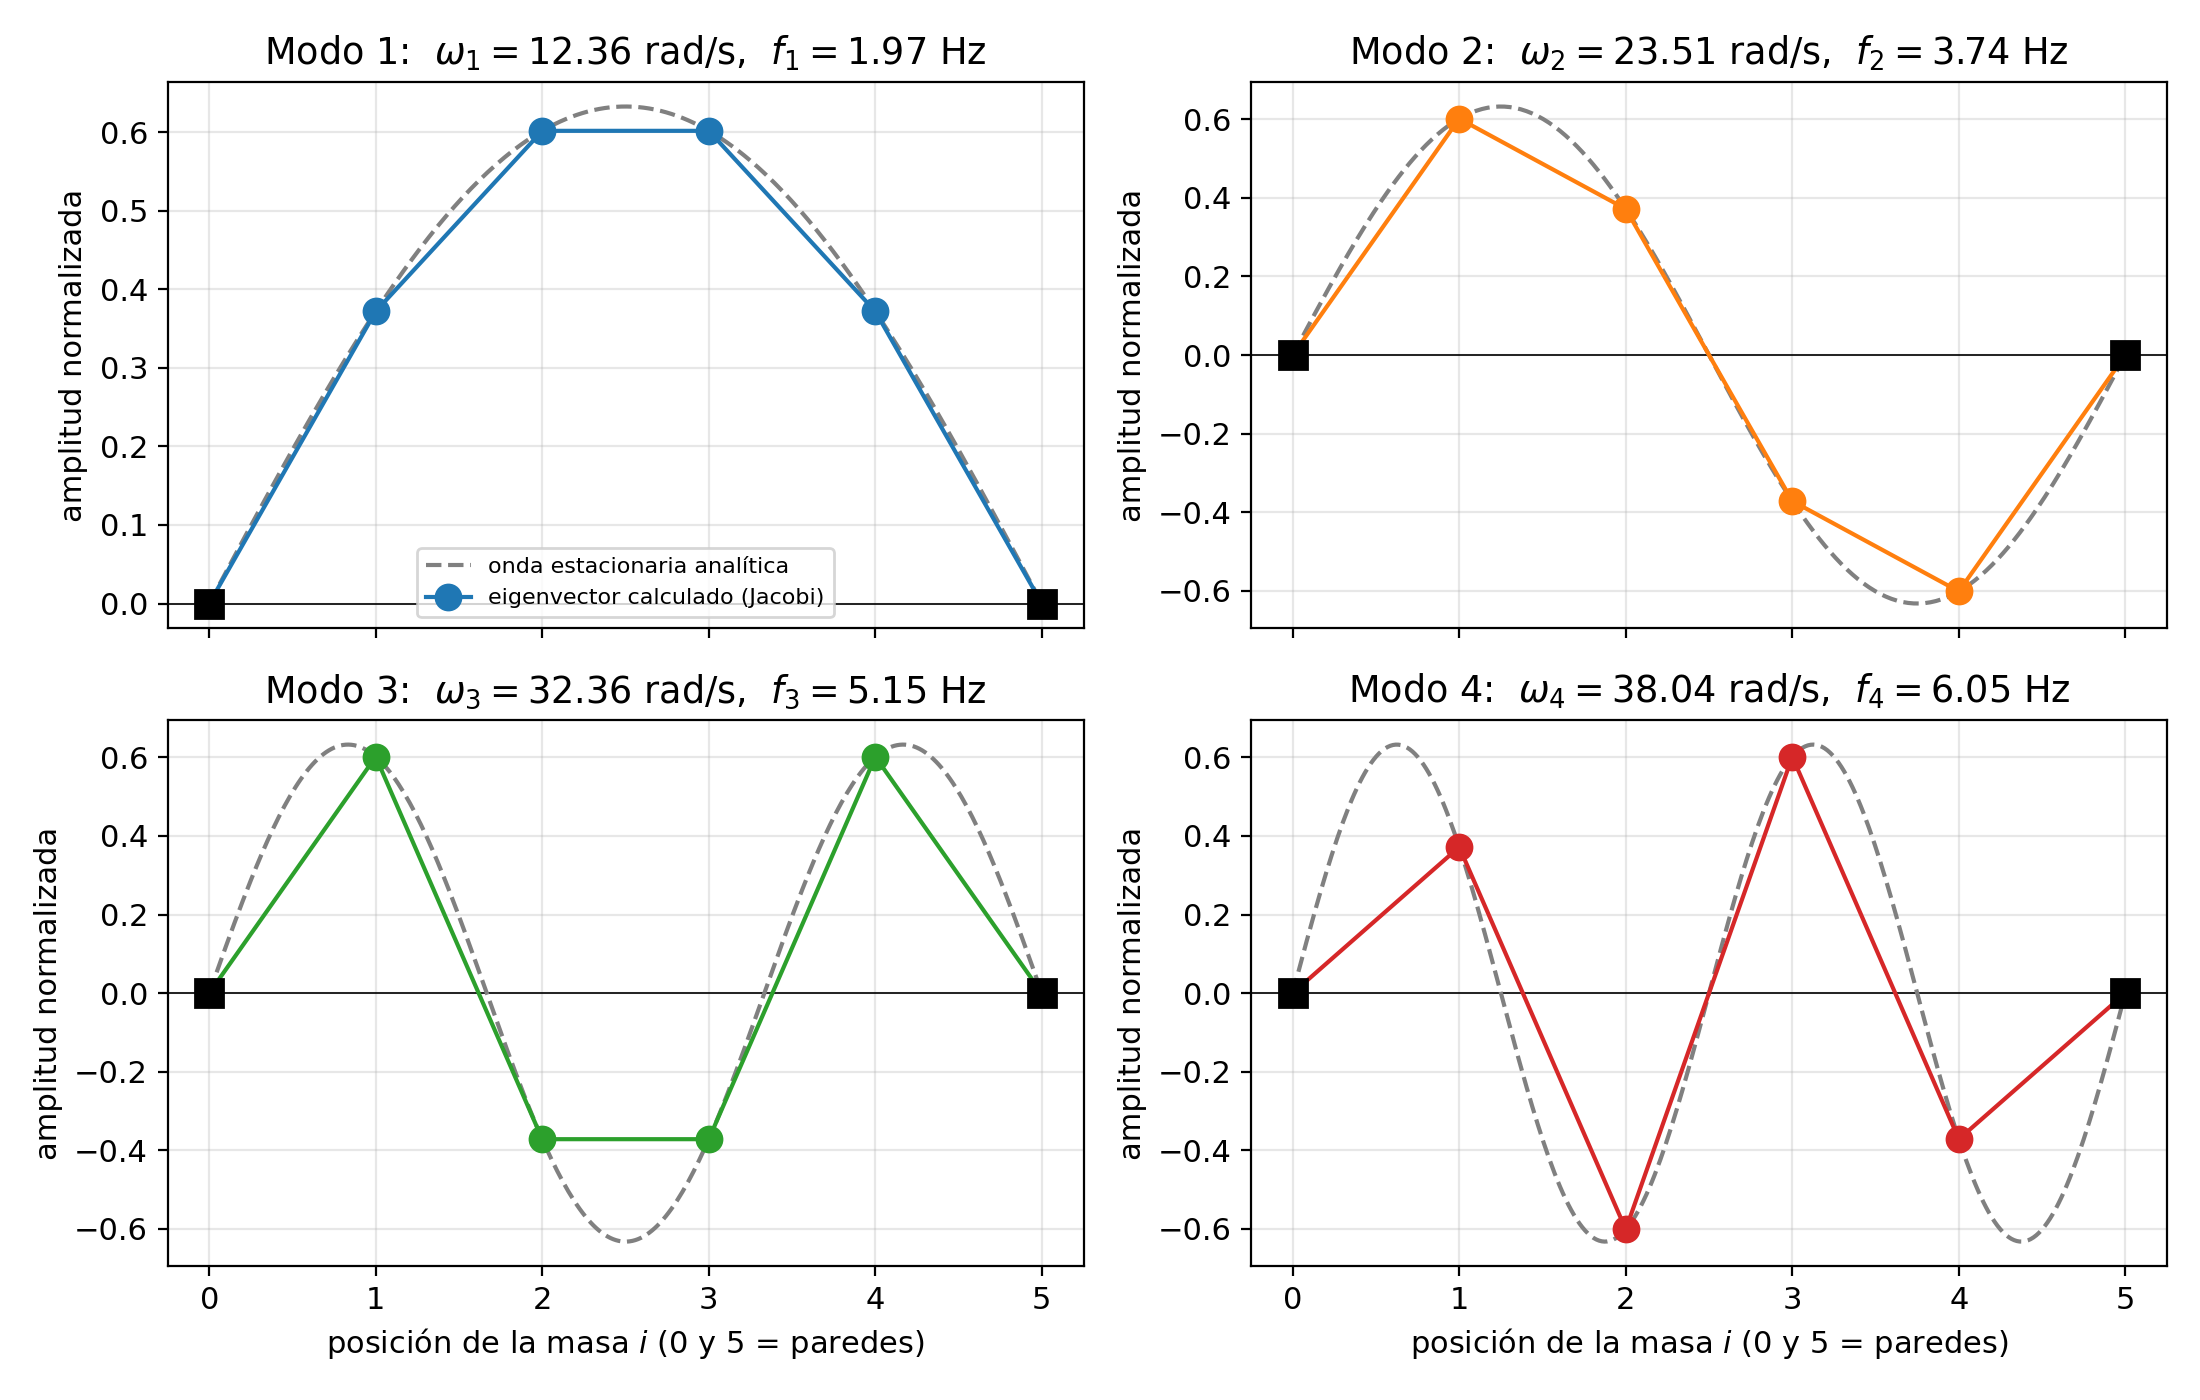
\includegraphics[width=.95\textwidth]{p2_modos.png}
\caption{Perfiles espaciales de los cuatro modos normales.}\label{fig:modos}
\end{figure}

Los modos permiten escribir el movimiento general. Como los eigenvectores son ortonormales y $M=mI$, la solución con velocidades iniciales nulas es $\vect x(t)=\sum_jc_j\vect v_j\cos\omega_jt$ con $c_j=\vect v_j^\top\vect x(0)$. Si la masa 1 se desplaza inicialmente, $c_j=v_{j,1}=(0.372,\,0.602,\,0.602,\,0.372)$; la Figura~\ref{fig:dinamica} muestra que la energía viaja de una masa a otra por interferencia entre modos de frecuencias distintas, algo que no ocurre en un modo aislado.

\begin{figure}[H]\centering
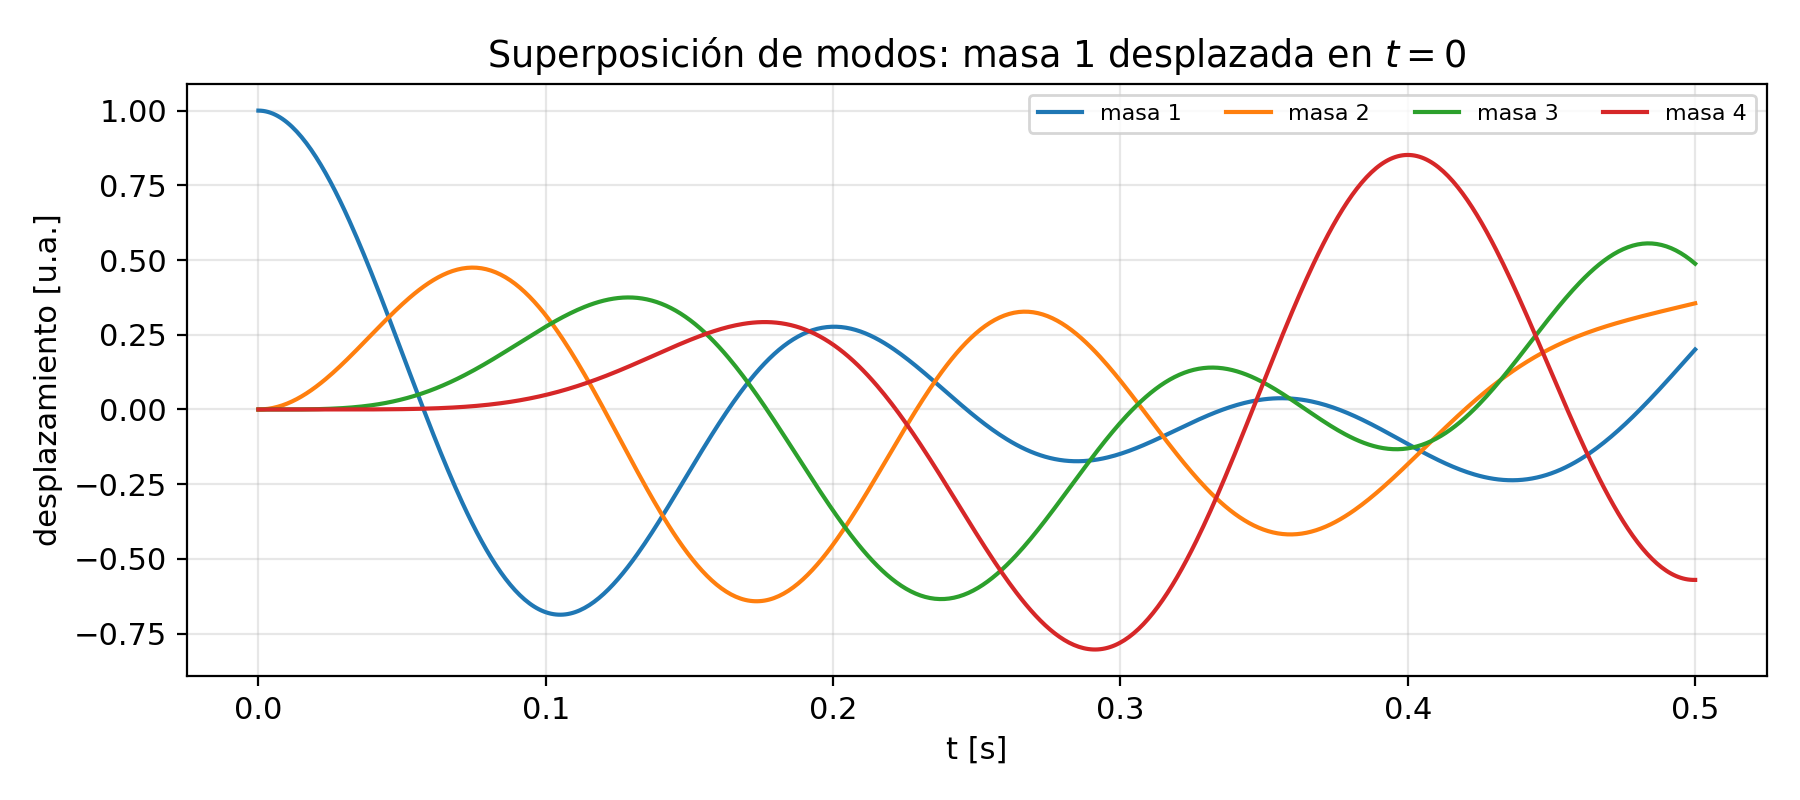
\includegraphics[width=.75\textwidth]{p2_dinamica.png}
\caption{Movimiento de las cuatro masas cuando solo la masa 1 se desplaza en $t=0$, reconstruido con los modos calculados.}\label{fig:dinamica}
\end{figure}

%=====================================================================
\section{Problema 3: ecuación de Kepler y dinámica orbital}
%=====================================================================
\paragraph{Planteamiento.}
Para un cuerpo en una órbita elíptica de semieje mayor $a$ y excentricidad $e$, la segunda ley de Kepler (ley de las áreas) implica que la anomalía media $M=n(t-\tau)$, con $n=2\pi/T_{\rm orb}$, crece linealmente con el tiempo, mientras que la posición geométrica se describe con la anomalía excéntrica $E$: $r=a(1-e\cos E)$ y $\tan(\nu/2)=\sqrt{(1+e)/(1-e)}\tan(E/2)$, donde $\nu$ es la anomalía verdadera. Ambas se relacionan mediante la ecuación trascendente
\begin{equation}
f(E)=E-e\sin E-M=0, \label{eq:kepler}
\end{equation}
que no puede resolverse de forma algebraica para $E$. Para $0<M<2\pi$ y $0\le e<1$, la función es continua con $f(0)=-M<0$ y $f(2\pi)=2\pi-M>0$; además $f'(E)=1-e\cos E\ge1-e>0$, luego $f$ es estrictamente creciente. En consecuencia existe una única raíz en $[0,2\pi]$ y la bisección está garantizada. Se usa $M=1.5$ rad ($85.9^\circ$).

\paragraph{Método de relajación (punto fijo) y análisis de convergencia.}
La ecuación~\eqref{eq:kepler} se reescribe como $E=g(E)=M+e\sin E$ y se itera $E_{k+1}=g(E_k)$ con $E_0=M$. Si $E^*$ es el punto fijo, restando $E^*=g(E^*)$ y aplicando el teorema del valor medio, $E_{k+1}-E^*=g'(\xi_k)(E_k-E^*)$ con $\xi_k$ entre $E_k$ y $E^*$. Por tanto, si $|g'|\le L<1$ en un entorno, la iteración es una contracción que converge linealmente:
\begin{equation}
|E_k-E^*|\le\frac{L^k}{1-L}|E_1-E_0|,\qquad \lim_{k\to\infty}\frac{E_{k+1}-E^*}{E_k-E^*}=g'(E^*)=e\cos E^*. \label{eq:contraccion}
\end{equation}
Aquí $|g'(E)|=|e\cos E|\le e<1$ para todo $E$, así que el método converge para cualquier semilla y cualquier $M$ (teorema de la contracción de Banach); la condición $|g'|<1$ pedida por el enunciado se cumple siempre. Sin embargo, la \emph{velocidad} depende de $\rho=|g'(E^*)|=e|\cos E^*|$: la cota $e$ es una garantía y el factor real puede ser bastante menor. Con la tolerancia $\varepsilon=10^{-6}$ sobre $|E_{k+1}-E_k|$ el número de iteraciones estimado a partir de~\eqref{eq:contraccion} es $k\gtrsim\ln\!\big[\varepsilon(1-\rho)/|E_1-E_0|\big]/\ln\rho$.

Con $M=1.5$ rad la raíz de referencia (bisección a $10^{-15}$) es $E^*=1.599957$ rad para $e=0.1$ y $E^*=2.228235$ rad para $e=0.92$. Los resultados son:

\begin{itemize}
\item \textbf{Órbita planetaria ($e=0.1$).} $\rho=0.1|\cos1.6|=2.9\times10^{-3}$: cada iteración gana casi tres cifras decimales, y bastan 3 iteraciones (Tabla~\ref{tab:rel01}). La estimación teórica es $\ln(10^{-5})/\ln(0.0029)\approx2$.
\item \textbf{Órbita cometaria ($e=0.92$).} $\rho=0.92|\cos2.228|=0.562$. Ahora se ganan $\log_{10}(1/0.562)=0.25$ cifras por iteración y se necesitan 24 iteraciones (Tabla~\ref{tab:rel092}), frente a $\approx25$ de la estimación teórica. El signo de $g'(E^*)$ es negativo, y por eso los iterados alternan a ambos lados de la raíz: la telaraña de la Figura~\ref{fig:tela} (derecha) es una espiral y no una escalera, y las razones $e_{k+1}/e_k$ convergen a $0.56$ (Tabla~\ref{tab:rel092}, columna $|g'(E_k)|$).
\end{itemize}

\begin{table}[H]\centering\small
\begin{tabular}{r c c c c}
\toprule
$k$ & $E_k$ [rad] & $|E_k-E_{k-1}|$ & $|E_k-E^*|$ & $|g'(E_k)|$\\
\midrule
0 & 1.50000000 & -- & 1.00e-01 & 0.0071\\
1 & 1.59974950 & 9.97e-02 & 2.08e-04 & 0.0029\\
2 & 1.59995809 & 2.09e-04 & 6.04e-07 & 0.0029\\
3 & 1.59995748 & 6.06e-07 & 1.76e-09 & 0.0029\\
\bottomrule
\end{tabular}

\caption{Relajación para $e=0.1$, $M=1.5$ rad ($E^*=1.599957$).}\label{tab:rel01}
\end{table}
\begin{table}[H]\centering\scriptsize
\begin{tabular}{r c c c c}
\toprule
$k$ & $E_k$ [rad] & $|E_k-E_{k-1}|$ & $|E_k-E^*|$ & $|g'(E_k)|$\\
\midrule
0 & 1.50000000 & -- & 7.28e-01 & 0.0651\\
1 & 2.41769539 & 9.18e-01 & 1.89e-01 & 0.6893\\
2 & 2.10932487 & 3.08e-01 & 1.19e-01 & 0.4718\\
3 & 2.28978714 & 1.80e-01 & 6.16e-02 & 0.6059\\
4 & 2.19227313 & 9.75e-02 & 3.60e-02 & 0.5357\\
5 & 2.24797794 & 5.57e-02 & 1.97e-02 & 0.5765\\
6 & 2.21699447 & 3.10e-02 & 1.12e-02 & 0.5540\\
7 & 2.23450856 & 1.75e-02 & 6.27e-03 & 0.5668\\
8 & 2.22469390 & 9.81e-03 & 3.54e-03 & 0.5596\\
9 & 2.23022148 & 5.53e-03 & 1.99e-03 & 0.5636\\
10 & 2.22711698 & 3.10e-03 & 1.12e-03 & 0.5614\\
11 & 2.22886333 & 1.75e-03 & 6.28e-04 & 0.5627\\
12 & 2.22788184 & 9.81e-04 & 3.53e-04 & 0.5619\\
13 & 2.22843373 & 5.52e-04 & 1.99e-04 & 0.5623\\
14 & 2.22812349 & 3.10e-04 & 1.12e-04 & 0.5621\\
15 & 2.22829792 & 1.74e-04 & 6.28e-05 & 0.5622\\
16 & 2.22819985 & 9.81e-05 & 3.53e-05 & 0.5622\\
17 & 2.22825499 & 5.51e-05 & 1.98e-05 & 0.5622\\
18 & 2.22822399 & 3.10e-05 & 1.12e-05 & 0.5622\\
19 & 2.22824142 & 1.74e-05 & 6.27e-06 & 0.5622\\
20 & 2.22823162 & 9.80e-06 & 3.53e-06 & 0.5622\\
21 & 2.22823713 & 5.51e-06 & 1.98e-06 & 0.5622\\
22 & 2.22823403 & 3.10e-06 & 1.11e-06 & 0.5622\\
23 & 2.22823577 & 1.74e-06 & 6.27e-07 & 0.5622\\
24 & 2.22823479 & 9.79e-07 & 3.52e-07 & 0.5622\\
\bottomrule
\end{tabular}

\caption{Relajación para $e=0.92$, $M=1.5$ rad ($E^*=2.228235$).}\label{tab:rel092}
\end{table}

\begin{figure}[H]\centering
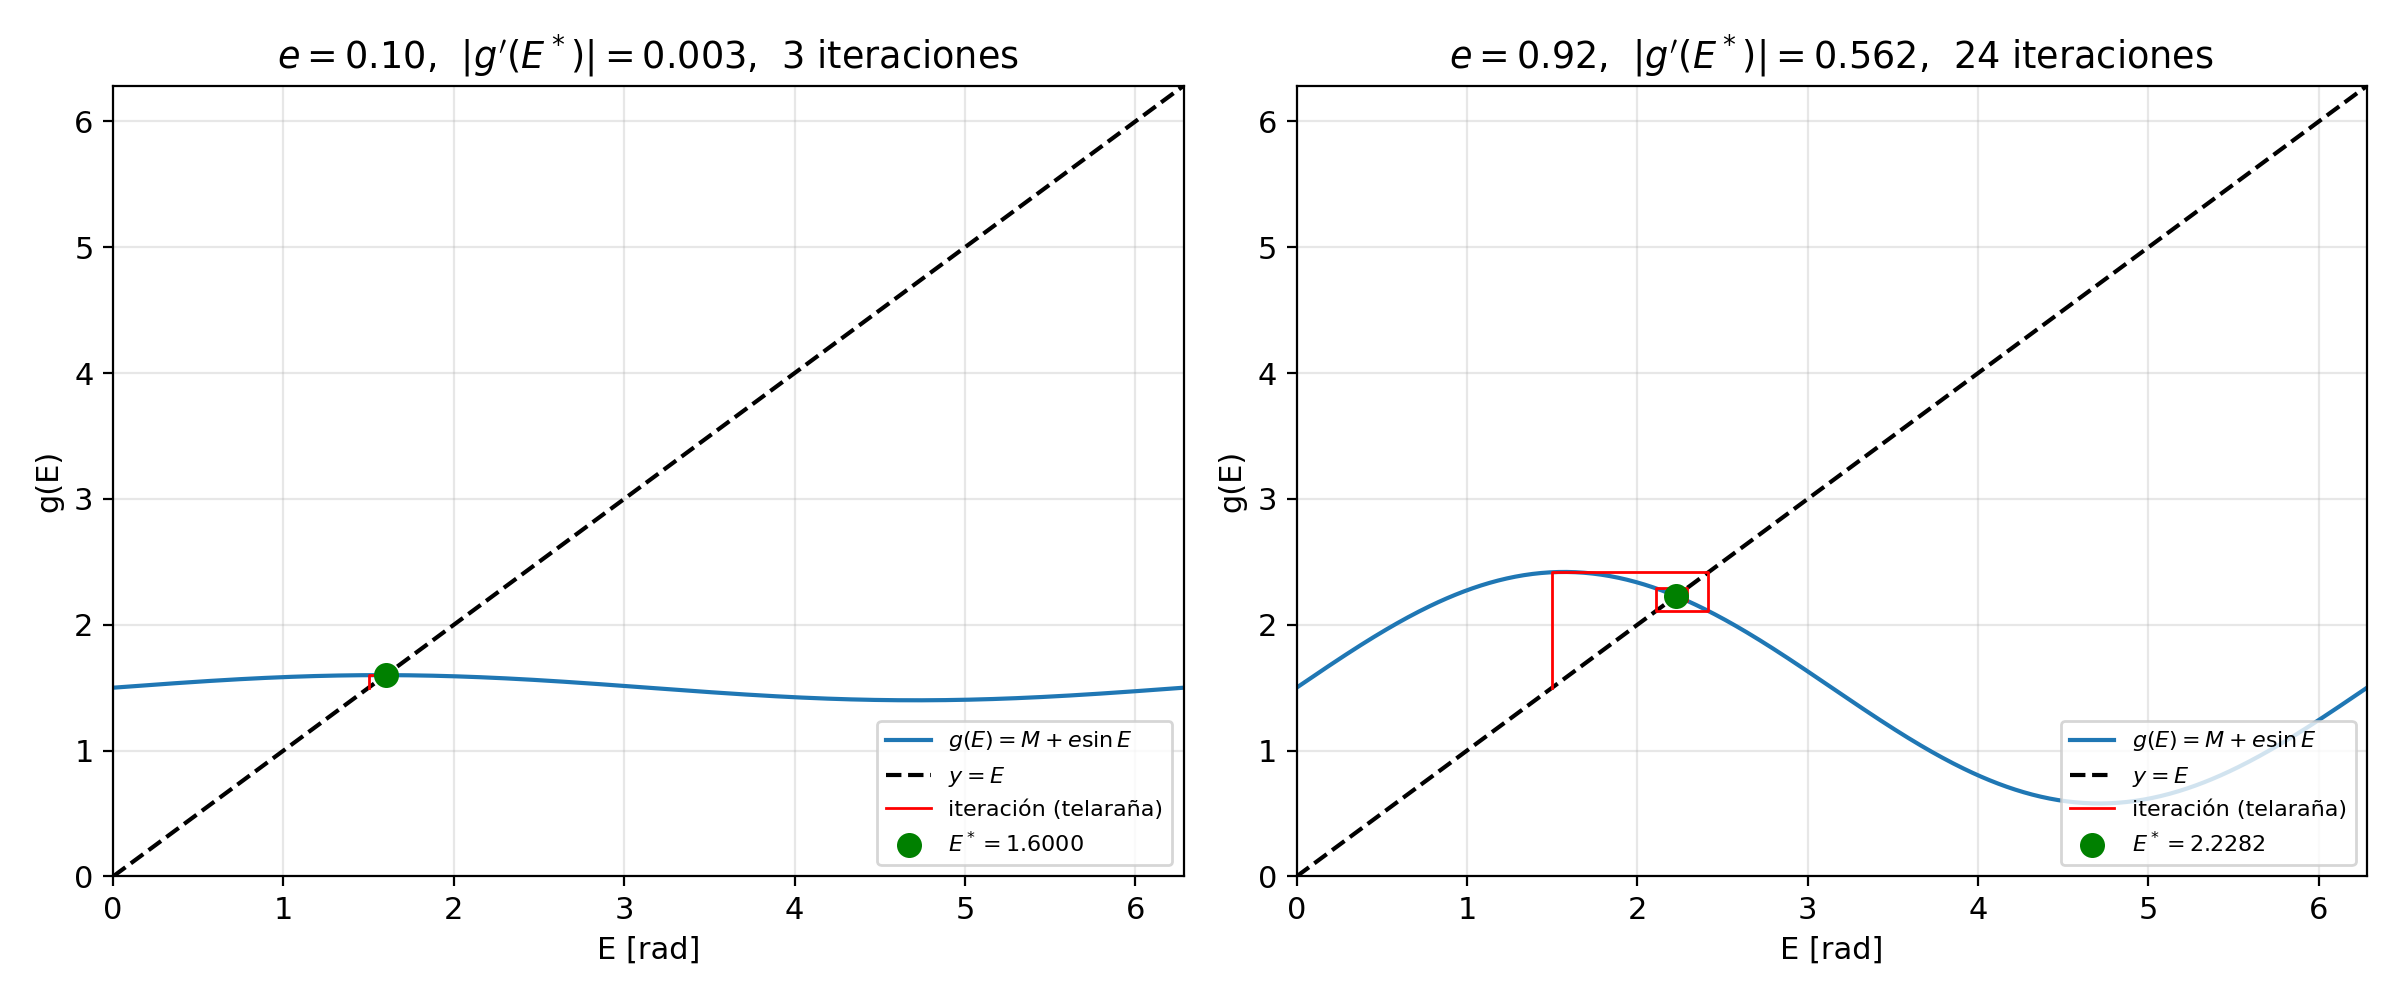
\includegraphics[width=\textwidth]{p3_telarana.png}
\caption{Diagrama de telaraña de la iteración $E_{k+1}=M+e\sin E_k$. Con $e=0.1$ la curva $g$ es casi plana y la iteración cae de inmediato sobre la raíz; con $e=0.92$ la pendiente en el punto fijo es mayor y la iteración espirala lentamente.}\label{fig:tela}
\end{figure}

Un caso todavía más desfavorable se da para $e=0.92$ y $M=0.1$ rad (cuerpo muy cerca del perihelio): entonces $E^*=0.6747$ y $\rho=0.92\cos(0.6747)\approx0.718$; se necesitan 41 iteraciones. La razón es geométrica: cerca del perihelio $\cos E^*$ está próximo a 1 y $|g'|$ se acerca a la cota $e$. La Figura~\ref{fig:p3err} (derecha) verifica que el error decae con la pendiente $\ln\rho$ predicha.

\begin{figure}[H]\centering
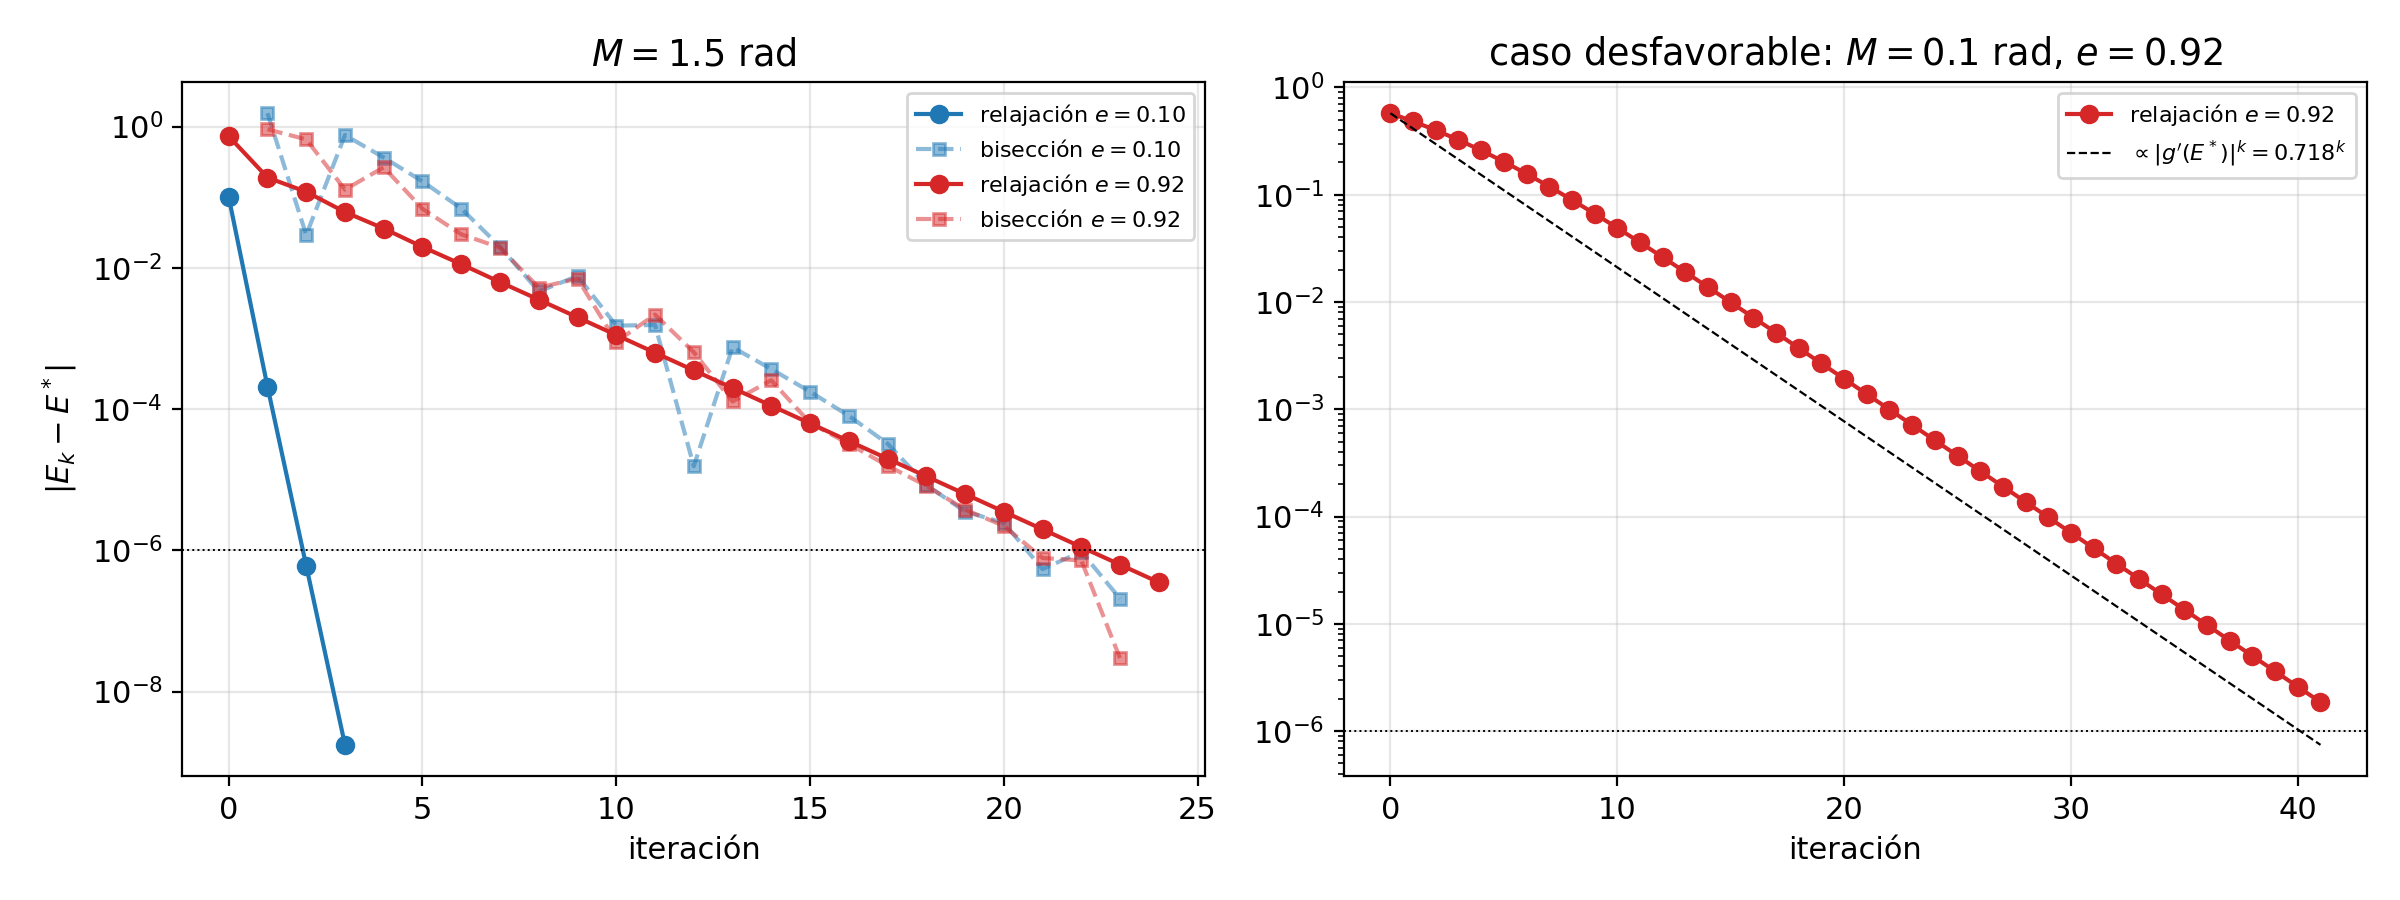
\includegraphics[width=\textwidth]{p3_error.png}
\caption{Error $|E_k-E^*|$ frente a la iteración (escala semilogarítmica). Izquierda: $M=1.5$ rad, relajación (círculos) y bisección (cuadrados). Derecha: caso desfavorable $M=0.1$, $e=0.92$, con la recta teórica $\rho^k$.}\label{fig:p3err}
\end{figure}

\paragraph{Búsqueda binaria (bisección) y comparación.}
La bisección parte de $[a,b]=[0,2\pi]$, con $f(a)<0<f(b)$. Cada iteración toma el punto medio $c=(a+b)/2$ y conserva la mitad en la que $f$ cambia de signo, de modo que tras $n$ pasos la incertidumbre es $(b-a)/2^n$. Para alcanzar $\varepsilon=10^{-6}$ se necesita
\begin{equation}
n\ge\log_2\frac{2\pi}{\varepsilon}=22.6\quad\Rightarrow\quad n=23, \label{eq:biseccion}
\end{equation}
independientemente de $e$ y de $M$: solo depende del ancho del intervalo inicial y de la tolerancia. Los 23 pasos observados en todos los casos lo confirman. El método es lineal con razón exacta $1/2$ en el peor caso, pero robusto y sin condiciones sobre $g'$. Las Tablas~\ref{tab:bis01} y~\ref{tab:bis092} muestran algunas iteraciones para las dos excentricidades. En la práctica, el error de la bisección no baja de forma monótona (puede aumentar entre iteraciones), aunque la cota $(b-a)/2^n$ sí lo hace; se ve en los cuadrados de la Figura~\ref{fig:p3err}.

\begin{table}[H]\centering\small
\begin{minipage}{.48\textwidth}\centering\begin{tabular}{r c c}
\toprule
$k$ & $E_k$ [rad] & $|E_k-E^*|$\\
\midrule
1 & 3.14159265 & 1.54e+00\\
2 & 1.57079633 & 2.92e-02\\
3 & 2.35619449 & 7.56e-01\\
4 & 1.96349541 & 3.64e-01\\
5 & 1.76714587 & 1.67e-01\\
6 & 1.66897110 & 6.90e-02\\
\vdots & \vdots & \vdots\\
21 & 1.59995694 & 5.42e-07\\
22 & 1.59995844 & 9.56e-07\\
23 & 1.59995769 & 2.07e-07\\
\bottomrule
\end{tabular}
\caption{Bisección, $e=0.1$.}\label{tab:bis01}\end{minipage}
\begin{minipage}{.48\textwidth}\centering\begin{tabular}{r c c}
\toprule
$k$ & $E_k$ [rad] & $|E_k-E^*|$\\
\midrule
1 & 3.14159265 & 9.13e-01\\
2 & 1.57079633 & 6.57e-01\\
3 & 2.35619449 & 1.28e-01\\
4 & 1.96349541 & 2.65e-01\\
5 & 2.15984495 & 6.84e-02\\
6 & 2.25801972 & 2.98e-02\\
\vdots & \vdots & \vdots\\
21 & 2.22823592 & 7.78e-07\\
22 & 2.22823443 & 7.20e-07\\
23 & 2.22823518 & 2.95e-08\\
\bottomrule
\end{tabular}
\caption{Bisección, $e=0.92$.}\label{tab:bis092}\end{minipage}
\end{table}

Para comparar ambos métodos en el rango completo $e\in[0.1,0.95]$ se contó el número de iteraciones para $\varepsilon=10^{-6}$ con paso $\Delta e=0.01$ (Figura~\ref{fig:p3it}, Tabla~\ref{tab:p3it}). Una iteración de cualquiera de los dos métodos cuesta una evaluación de $\sin$, por lo que el número de iteraciones es una medida directa del coste.

\begin{figure}[H]\centering
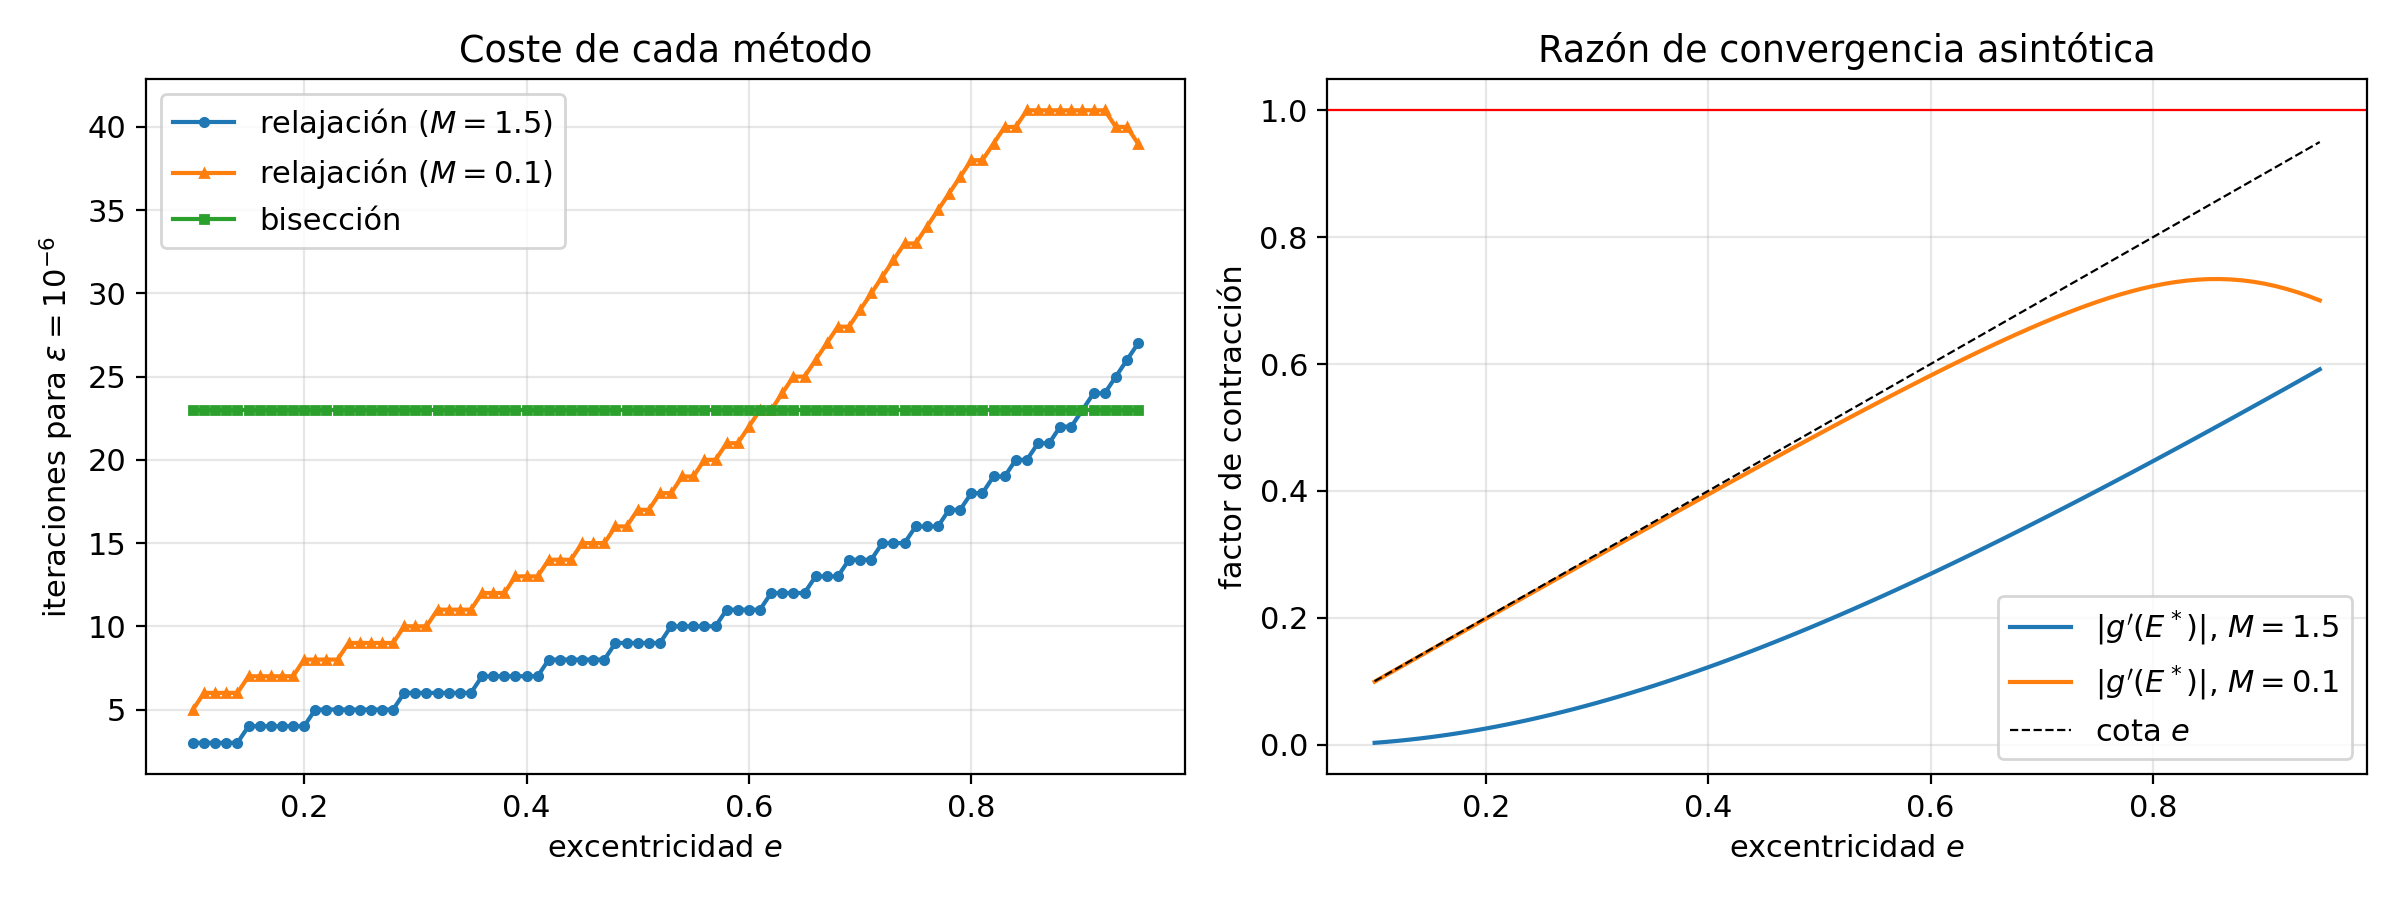
\includegraphics[width=\textwidth]{p3_iteraciones.png}
\caption{Izquierda: iteraciones necesarias para $\varepsilon=10^{-6}$ en función de $e$. Derecha: factor de contracción $|g'(E^*)|$, siempre por debajo de la cota $e$.}\label{fig:p3it}
\end{figure}
\begin{table}[H]\centering\small
\begin{tabular}{c cc cc c}
\toprule
 & \multicolumn{2}{c}{$M=1.5$ rad} & \multicolumn{2}{c}{$M=0.1$ rad} & \\
$e$ & relajación & $|g'(E^*)|$ & relajación & $|g'(E^*)|$ & bisección\\
\midrule
0.10 & 3 & 0.003 & 5 & 0.099 & 23\\
0.30 & 6 & 0.066 & 10 & 0.297 & 23\\
0.50 & 9 & 0.191 & 17 & 0.490 & 23\\
0.70 & 14 & 0.355 & 29 & 0.664 & 23\\
0.80 & 18 & 0.447 & 38 & 0.723 & 23\\
0.90 & 23 & 0.543 & 41 & 0.727 & 23\\
0.92 & 24 & 0.562 & 41 & 0.718 & 23\\
0.95 & 27 & 0.592 & 39 & 0.700 & 23\\
\bottomrule
\end{tabular}

\caption{Iteraciones de cada método para distintas excentricidades y anomalías medias.}\label{tab:p3it}
\end{table}

Con $M=1.5$ la relajación es más rápida que la bisección hasta $e=0.90$ (donde empatan, con 23 iteraciones) y la supera a partir de $e=0.91$; con $M=0.1$ el cruce ocurre ya en $e=0.63$. La bisección es constante (23 iteraciones) y la relajación crece aproximadamente como $\ln\varepsilon/\ln\rho$ con $\rho\to e|\cos E^*|$. La regla práctica es que la relajación gana cuando $\rho<1/2$, y la bisección cuando $\rho>1/2$. En órbitas de alta excentricidad y cerca del perihelio conviene un método de convergencia más rápida (Newton o Halley, o un arranque mejor de la relajación); en órbitas casi circulares, la relajación con $E_0=M$ es casi inmediata. Como la ecuación aparece en cada paso de tiempo de una simulación orbital, este análisis explica por qué los códigos de mecánica celeste usan Newton con una buena semilla para $e$ grande.

Para completar el sentido físico, con $M=1.5$ rad se obtiene para $e=0.1$: $r/a=1.0029$ y $\nu=1.700$ rad ($97.4^\circ$), casi igual a la posición sobre una circunferencia; para $e=0.92$: $r/a=1.562$ y $\nu=2.942$ rad ($168.5^\circ$). En ambos casos ha transcurrido el mismo $24\,\%$ del período ($M/2\pi$), pero el planeta ha barrido el $27\,\%$ del ángulo completo y el cometa el $47\,\%$. Esto es la segunda ley de Kepler: cerca del perihelio el cuerpo barre ángulo muy rápido y luego se demora en la parte lejana de la órbita (Figura~\ref{fig:orbita}).

\begin{figure}[H]\centering
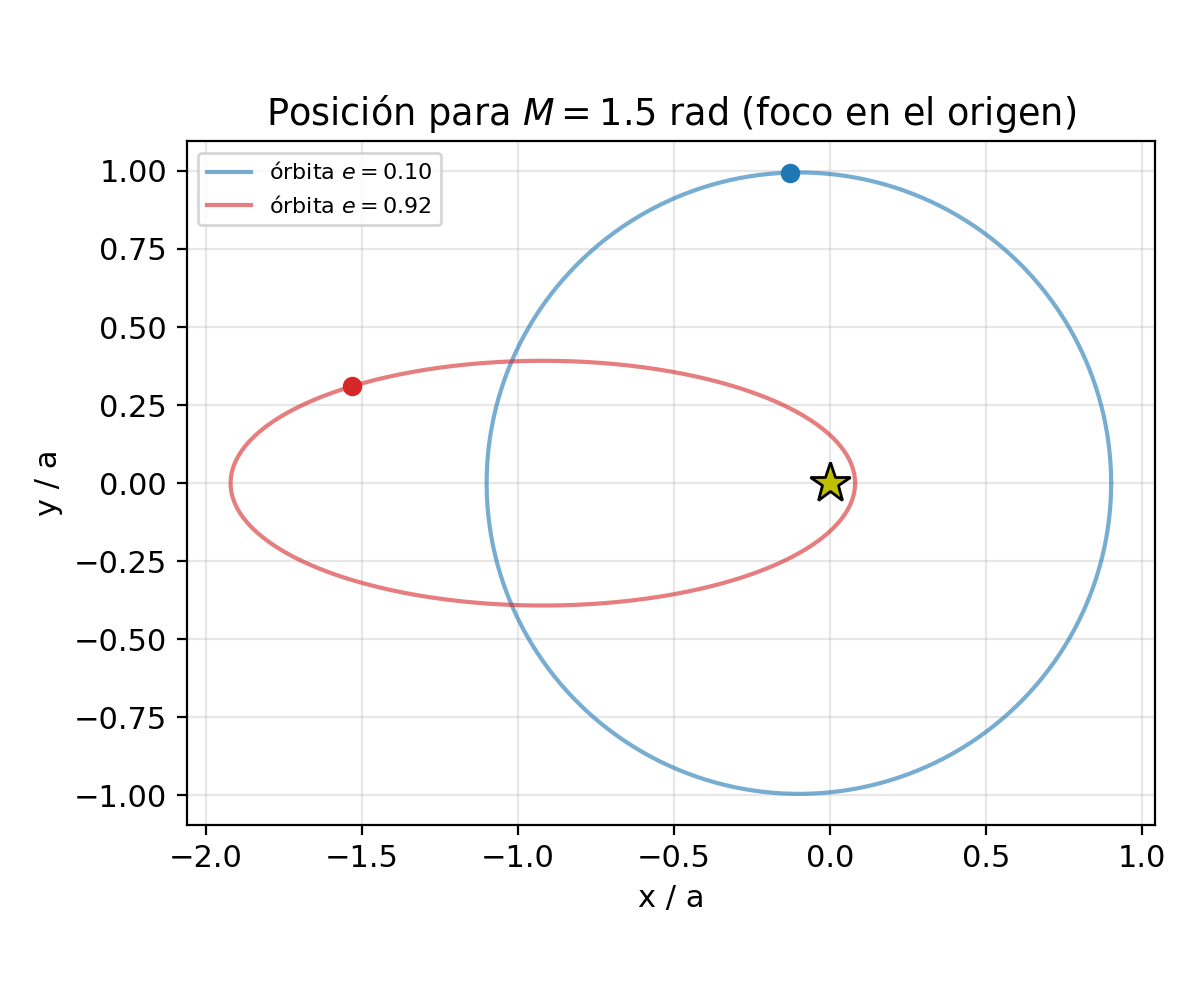
\includegraphics[width=.55\textwidth]{p3_orbita.png}
\caption{Posición del cuerpo para $M=1.5$ rad en las dos órbitas (el Sol está en el foco, en el origen).}\label{fig:orbita}
\end{figure}

%=====================================================================
\section{Problema 4: termodinámica real y sistemas no lineales multivariables}
%=====================================================================
\paragraph{Parte A: volumen molar de un gas de Van der Waals.}
La ecuación de estado de Van der Waals corrige la del gas ideal con dos efectos: el volumen propio de las moléculas ($v\to v-b$) y la atracción entre ellas, que reduce la presión en $a/v^2$. El volumen molar a $P=2\times10^6$ Pa y $T=300$ K es la raíz de
\begin{equation}
f(v)=\Big(P+\frac a{v^2}\Big)(v-b)-RT=0,\qquad a=0.3643\ \mathrm{Pa\,m^6/mol^2},\ b=4.267\times10^{-5}\ \mathrm{m^3/mol}, \label{eq:vdw}
\end{equation}
con $R=8.314462618$ J/(mol\,K), es decir $RT=2494.34$ J/mol. La derivada, necesaria para Newton, es
\[
f'(v)=\Big(P+\frac a{v^2}\Big)-\frac{2a(v-b)}{v^3}=P-\frac a{v^2}+\frac{2ab}{v^3}.
\]
Con los parámetros críticos $P_c=a/(27b^2)=7.41$ MPa y $T_c=8a/(27Rb)=304.25$ K se comprueba que el estado es $T_r=0.986$ y $P_r=0.270$, un gas comprimido por debajo del punto crítico. Como a $T<T_c$ la isoterma de Van der Waals puede tener tres raíces, se rastreó el signo de $f$ en $(b,0.1)$ m$^3$/mol con 20\,000 puntos: hay un único cambio de signo, cerca de $1.135\times10^{-3}$ m$^3$/mol, así que la raíz es única (el estado está lejos del lazo de coexistencia). La semilla natural es el gas ideal, $v_0=RT/P=1.24717\times10^{-3}$ m$^3$/mol.

\textbf{Método de Newton.} Se linealiza $f$ alrededor de $v_k$ y se anula la recta tangente, $v_{k+1}=v_k-f(v_k)/f'(v_k)$. El desarrollo de Taylor de $f$ en torno a $v^*$ muestra que el error cumple $e_{k+1}\approx\dfrac{f''(v^*)}{2f'(v^*)}e_k^2$: convergencia cuadrática (el número de cifras correctas se duplica en cada paso). \textbf{Método de la secante.} Sustituye $f'(v_k)$ por el cociente incremental,
\[
v_{k+1}=v_k-f(v_k)\frac{v_k-v_{k-1}}{f(v_k)-f(v_{k-1})},
\]
no requiere derivada, y su error cumple $e_{k+1}\approx\big|\tfrac{f''}{2f'}\big|\,e_k\,e_{k-1}$; si $e_{k+1}\sim Ce_k^{p}$ esto obliga a $p^2=p+1$, es decir $p=\phi=\tfrac{1+\sqrt5}2=1.618$ (superlineal), con constante $\big|\tfrac{f''}{2f'}\big|^{\phi-1}$. Como semillas se usan $v_0=RT/P$ para ambos y $v_1=1.05\,v_0$ para la secante.

\textbf{Precisión aritmética.} Con aritmética de doble precisión el error se estanca en $\sim10^{-19}$ m$^3$/mol (el paso de Newton sería inferior a la resolución de la máquina), lo que impediría observar el tercer y el cuarto ciclo de duplicación de cifras. Por eso este experimento, y solo este, se hizo con los mismos algoritmos ejecutados con números \texttt{Decimal} de 80 dígitos de la biblioteca estándar de Python (la lógica de \texttt{newton\_1d} y \texttt{secante} no cambia, solo el tipo numérico). La raíz que se obtiene es
\[
v^*=1.13544655460\times10^{-3}\ \mathrm{m^3/mol},\qquad |f(v^*)|<10^{-75},
\]
por ambos métodos, con coincidencia hasta el último de los 80 dígitos. La Tabla~\ref{tab:ns} da el error absoluto frente a la iteración y la Figura~\ref{fig:vdw} lo grafica en escala semilogarítmica.

\begin{table}[H]\centering\small
\resizebox{\textwidth}{!}{\begin{tabular}{r cc cc}
\toprule
 & \multicolumn{2}{c}{Newton} & \multicolumn{2}{c}{Secante}\\
$k$ & $v_k$ [m$^3$/mol] & $e_k=|v_k-v^*|$ & $v_k$ [m$^3$/mol] & $e_k=|v_k-v^*|$\\
\midrule
0 & 1.247169392700e-03 & 1.12e-04 & 1.247169392700e-03 & 1.12e-04\\
1 & 1.136738360037e-03 & 1.29e-06 & 1.309527862335e-03 & 1.74e-04\\
2 & 1.135446765995e-03 & 2.11e-10 & 1.137356283771e-03 & 1.91e-06\\
3 & 1.135446554598e-03 & 5.68e-18 & 1.135482606357e-03 & 3.61e-08\\
4 & 1.135446554598e-03 & 4.09e-33 & 1.135446563325e-03 & 8.73e-12\\
5 & 1.135446554598e-03 & 2.12e-63 & 1.135446554598e-03 & 4.00e-17\\
6 & 1.135446554598e-03 & $<10^{-60}$ & 1.135446554598e-03 & 4.43e-26\\
7 &  &  & 1.135446554598e-03 & 2.25e-40\\
8 &  &  & 1.135446554598e-03 & 1.26e-63\\
\bottomrule
\end{tabular}
}
\caption{Error absoluto $e_k=|v_k-v^*|$ para Newton y secante (aritmética de 80 dígitos).}\label{tab:ns}
\end{table}

En la Tabla~\ref{tab:ns} el error de Newton pasa de $1.1\times10^{-4}$ a $1.3\times10^{-6}$, $2.1\times10^{-10}$, $5.7\times10^{-18}$, $4.1\times10^{-33}$ y $2.1\times10^{-63}$: los exponentes se duplican aproximadamente en cada paso (6, 10, 18, 33, 63), la firma de la convergencia cuadrática. La secante necesita $8$ iteraciones para bajar de $10^{-62}$ frente a $5$ de Newton, y sus exponentes (6, 8, 12, 17, 26, 40, 63) crecen por el factor $\phi=1.618$ y no por 2. Además, la segunda semilla de la secante, $v_1=1.05\,v_0$ (fila $k=1$), está más lejos de la raíz ($1.7\times10^{-4}$) que la primera ($1.1\times10^{-4}$): es un arranque deliberadamente malo que sirve para ver que la secante, a diferencia de Newton, necesita dos semillas y tarda unas iteraciones en «encontrar» su régimen asintótico.

\begin{table}[H]\centering\small
\begin{tabular}{r cc cc}
\toprule
 & \multicolumn{2}{c}{Newton} & \multicolumn{2}{c}{Secante}\\
$k$ & $e_{k+1}/e_k^{2}$ & $p_k$ & $e_{k+1}/e_k^{1.618}$ & $p_k$\\
\midrule
1 & 126.6792 & 1.955 & 2.3097 & -10.175\\
2 & 126.9969 & 2.000 & 64.6411 & 0.880\\
3 & 126.9970 & 2.000 & 9.6387 & 2.097\\
4 & -- & 2.000 & 31.3056 & 1.477\\
5 & -- & -- & 15.1164 & 1.677\\
6 & -- & -- & 23.7058 & 1.596\\
\bottomrule
\end{tabular}

\caption{Constante asintótica y orden de convergencia estimado con~\eqref{eq:orden}.}\label{tab:orden}
\end{table}

La Tabla~\ref{tab:orden} confirma el orden. Para Newton, $p_k=1.955,\,2.000,\,2.000,\,2.000$ y el cociente $e_{k+1}/e_k^2$ tiende a $126.997$, que coincide con la constante teórica $f''(v^*)/(2f'(v^*))=4.416\times10^{8}/(2\cdot1.7387\times10^{6})=126.997$. Para la secante, $p_k$ oscila al principio (los tres primeros valores no son representativos, por el paso inicial fallido) y se estabiliza en $1.48,\,1.68,\,1.60$ y $1.63$ (este último, $k=7$, fuera de la tabla), alrededor de $\phi=1.618$; la constante asintótica teórica es $126.997^{0.618}\approx20$, coherente con la última columna.

Sin embargo, el orden no basta para comparar coste: Newton evalúa $f$ y $f'$ en cada iteración (dos evaluaciones), la secante solo $f$ (una). El índice de eficiencia $p^{1/w}$ ($w$ = evaluaciones por iteración) es $\sqrt2=1.414$ para Newton y $1.618$ para la secante, luego la secante es más eficiente por evaluación cuando la derivada es costosa, aunque necesite más iteraciones.

\begin{figure}[H]\centering
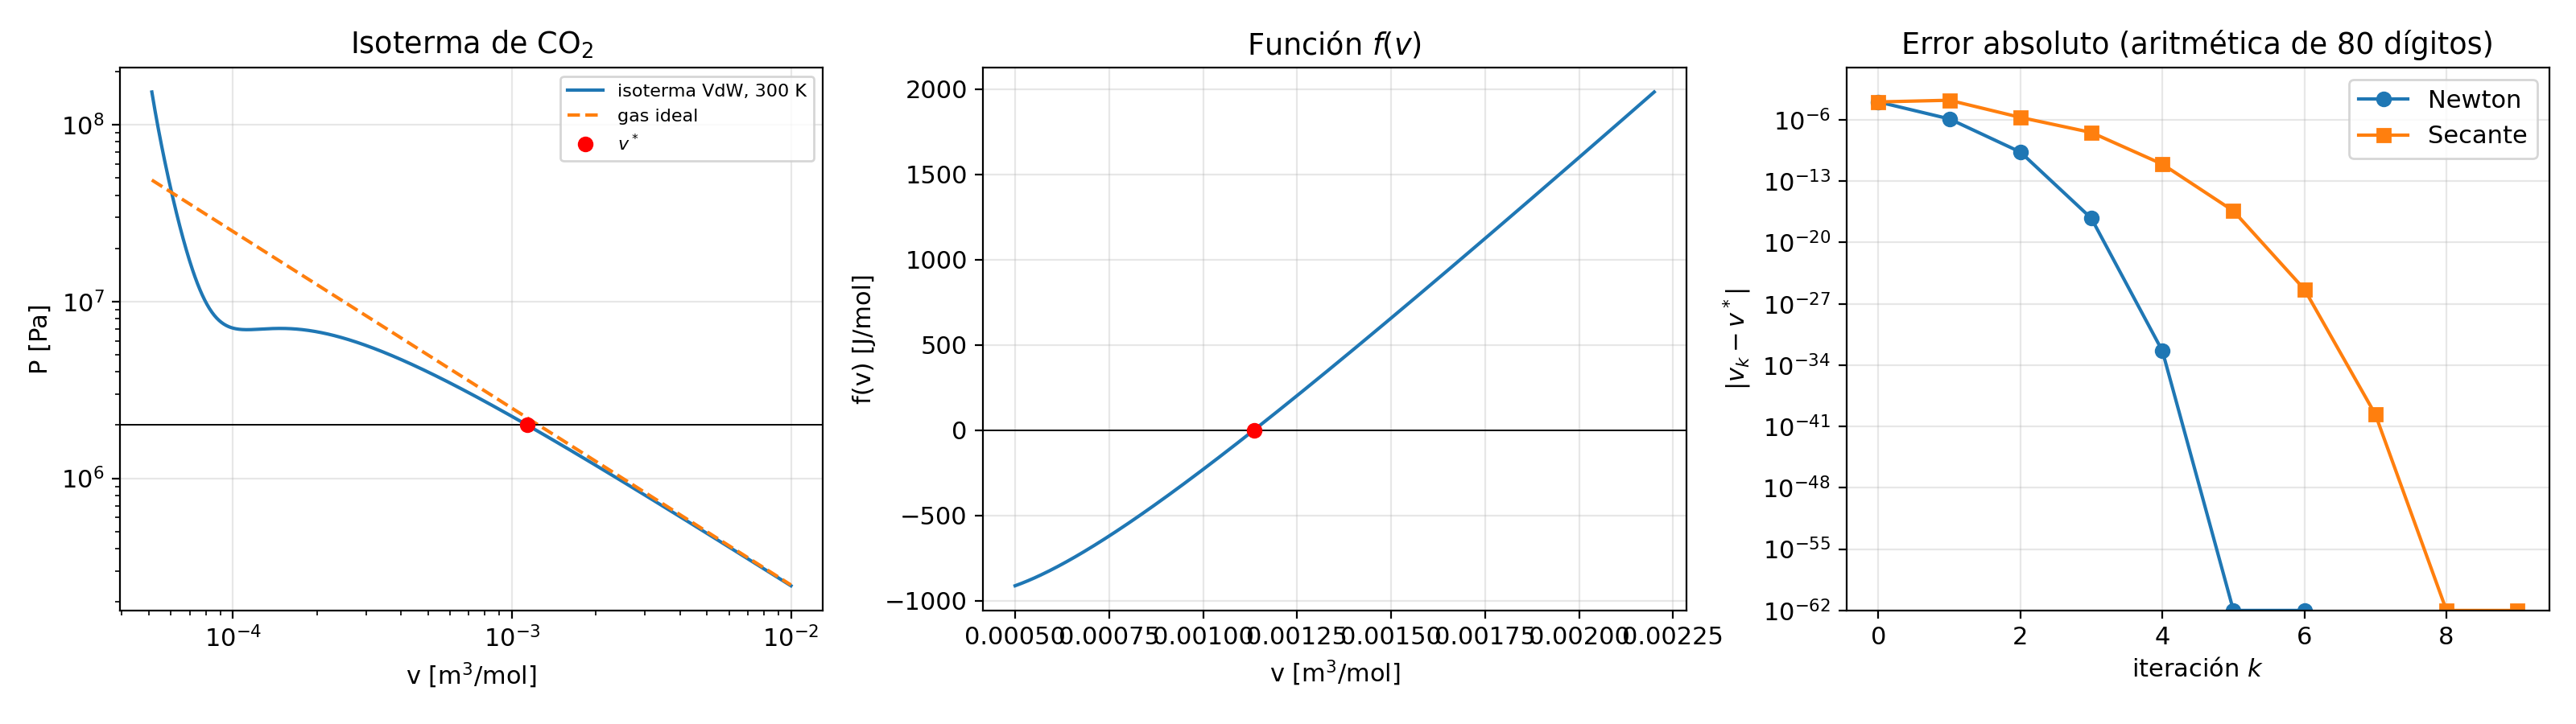
\includegraphics[width=\textwidth]{p4a_vdw.png}
\caption{Izquierda: isoterma de Van der Waals a 300 K frente a la ideal; el punto rojo es $v^*$. Centro: $f(v)$ con su cero. Derecha: error absoluto frente a la iteración.}\label{fig:vdw}
\end{figure}

\textbf{Interpretación física.} El volumen molar del gas real, $v^*=1.1354\times10^{-3}$ m$^3$/mol, es un 9\,\% menor que el del gas ideal ($1.2472\times10^{-3}$); el factor de compresibilidad es $Z=Pv^*/RT=0.9104$. Esto se entiende descomponiendo $Z=\dfrac v{v-b}-\dfrac a{RTv}=1.0391-0.1286$: la repulsión de corto alcance (volumen excluido) contribuye con $+3.9\,\%$ y la atracción de largo alcance con $-12.9\,\%$, y a esta temperatura, próxima a la crítica, la atracción domina. Un desarrollo del virial truncado, $Z\approx1+(b-a/RT)P/RT=0.9171$, da un valor cercano, pero no idéntico, porque a $2$ MPa el término siguiente ya no es despreciable.

\paragraph{Parte B: sistema no lineal $2\times2$.}
El sistema
\begin{equation}
f_1=x^3-3xy^2-1=0,\qquad f_2=3x^2y-y^3=0 \label{eq:sis2d}
\end{equation}
tiene una estructura oculta: con $z=x+iy$, $z^3=(x^3-3xy^2)+i(3x^2y-y^3)$, de modo que $f_1=\operatorname{Re}(z^3-1)$ y $f_2=\operatorname{Im}(z^3-1)$. Resolver el sistema es entonces resolver $z^3=1$, y sus tres raíces son las raíces cúbicas de la unidad:
\[
(x,y)=(1,0),\qquad\Big(-\tfrac12,\ +\tfrac{\sqrt3}2\Big),\qquad\Big(-\tfrac12,\ -\tfrac{\sqrt3}2\Big).
\]
Físicamente, $\operatorname{Re}z^3$ e $\operatorname{Im}z^3$ son funciones armónicas conjugadas (el potencial y la función de corriente de un campo de sextupolo, $n=3$), y las curvas $f_1=0$ y $f_2=0$ de la Figura~\ref{fig:sis2d} (izquierda) son sus equipotenciales; las intersecciones son las tres soluciones. Esta forma compacta da una solución analítica con la que verificar todos los resultados numéricos, aunque los algoritmos que siguen trabajan en $\mathbb R^2$ sin usar números complejos. También explica la Jacobiana del enunciado: las ecuaciones de Cauchy--Riemann $\partial_xf_1=\partial_yf_2$ y $\partial_yf_1=-\partial_xf_2$ dan a $J$ la estructura $\bigl(\begin{smallmatrix}\alpha&-\beta\\\beta&\alpha\end{smallmatrix}\bigr)$, con $\alpha+i\beta=3z^2$; es una matriz de «rotación por escala» equivalente a multiplicar por el número complejo $3z^2$, y $\det J=9|z|^4$.

\textbf{Relajación de dos variables.} Se busca un mapa de punto fijo $x_{k+1}=g_1(x_k,y_k)$, $y_{k+1}=g_2(x_{k+1},y_k)$ (esquema de Gauss--Seidel, que usa el $x$ recién calculado en la segunda ecuación). La forma más simple consiste en sumar a cada variable un múltiplo de su ecuación (subrelajación):
\begin{equation}
g_1(x,y)=x-\omega\,f_1(x,y),\qquad g_2(x,y)=y-\omega\,f_2(x,y),\qquad 0<\omega, \label{eq:rel2d}
\end{equation}
y el punto fijo de \eqref{eq:rel2d} satisface $f_1=f_2=0$. Su convergencia local se controla con la matriz de iteración $T=\partial(g_1,g_2)/\partial(x,y)$ en la raíz: hay convergencia si el radio espectral es $\rho(T)<1$. Con $\omega$ constante y $J$ evaluada en la raíz $z_0$, el esquema de Jacobi tiene eigenvalores $1-3\omega z_0^2$; en la raíz $(1,0)$ ($3z_0^2=3$) son iguales a $1-3\omega$, luego converge si $0<\omega<2/3$, y el óptimo es $\omega=1/3$. Con el esquema de Gauss--Seidel de \eqref{eq:rel2d} y $\omega=0.2$ se obtiene $\rho=0.4$ en $(1,0)$, que es el valor $|1-3\omega|$. En las otras dos raíces $3z_0^2=3e^{\pm4\pi i/3}$ no es real y $|1-3\omega z_0^2|>1$ para cualquier $\omega>0$ (y $\rho=1.3$ con $\omega=0.2$): estas raíces son repulsivas para \eqref{eq:rel2d}. Ello obliga a girar el paso: usar $x_{k+1}=x_k-\omega(\cos\theta\,f_1-\sin\theta\,f_2)$, $y_{k+1}=y_k-\omega(\sin\theta\,f_1+\cos\theta\,f_2)$ (evaluadas con $x_{k+1}$ en la segunda), es decir, multiplicar por $\omega e^{i\theta}$ y no por $\omega$; con $\theta=2\pi/3$ o $4\pi/3$ el factor pasa a ser $1-3\omega z_0^2e^{i\theta}$, cuyo módulo es $0.4$ en la raíz correspondiente. Así, un «$g$» distinto por raíz es lo que caracteriza a los métodos de relajación en varias variables.

Los resultados con $\omega=0.2$ son los siguientes. Desde $(1.4,\,0.4)$ y $\theta=0$ el método converge a $(1,\,0)$ en 30 iteraciones hasta un cambio de $10^{-12}$ (Tabla~\ref{tab:rel2d}); el error decae con razón $0.40$, exactamente el radio espectral predicho, como se ve en la Figura~\ref{fig:sis2d} (derecha) donde se superpone la recta $|1-3\omega|^k$. Con $\theta=2\pi/3$ desde $(-0.3,\,0.6)$ se llega a $(-0.5,\,0.866025)$ en 31 iteraciones, y con $\theta=4\pi/3$ desde $(-0.3,\,-0.6)$ a $(-0.5,\,-0.866025)$ en 31. Con $\theta=0$ desde $(-0.3,\,0.6)$ el método sigue convergiendo a $(1,0)$ (35 iteraciones): el punto de partida está en la cuenca de atracción de esa raíz, y las raíces repulsivas no pueden alcanzarse.

\begin{table}[H]\centering\small
\begin{tabular}{r c c c}
\toprule
$k$ & $x_k$ & $y_k$ & $\|(x_k,y_k)-(1,0)\|$\\
\midrule
0 & 1.4000000000 & 0.4000000000 & 5.66e-01\\
1 & 1.1856000000 & 0.0754446336 & 2.00e-01\\
2 & 1.0563418828 & 0.0250192115 & 6.16e-02\\
3 & 1.0209930753 & 0.0093739249 & 2.30e-02\\
4 & 1.0081847833 & 0.0036572897 & 8.96e-03\\
5 & 1.0032417004 & 0.0014486756 & 3.55e-03\\
6 & 1.0012916315 & 0.0005772240 & 1.41e-03\\
7 & 1.0005158513 & 0.0002305322 & 5.65e-04\\
10 & 1.0000329826 & 0.0000147398 & 3.61e-05\\
15 & 1.0000003377 & 0.0000001509 & 3.70e-07\\
20 & 1.0000000035 & 0.0000000015 & 3.79e-09\\
25 & 1.0000000000 & 0.0000000000 & 3.88e-11\\
30 & 1.0000000000 & 0.0000000000 & 3.97e-13\\
\bottomrule
\end{tabular}

\caption{Relajación de dos variables ($\theta=0$, $\omega=0.2$) desde $(1.4,\,0.4)$. La distancia a la raíz se reduce por un factor $\approx0.4$ en cada iteración.}\label{tab:rel2d}
\end{table}

La Figura~\ref{fig:omega} muestra la sensibilidad de la relajación a $\omega$: el radio espectral $|1-3\omega|$ vale $1$ en $\omega=2/3$ y se anula en $\omega=1/3$, donde la convergencia es más rápida; para $\omega$ pequeño el método es estable pero lento y cerca de $2/3$ oscila y casi no avanza.

\begin{figure}[H]\centering
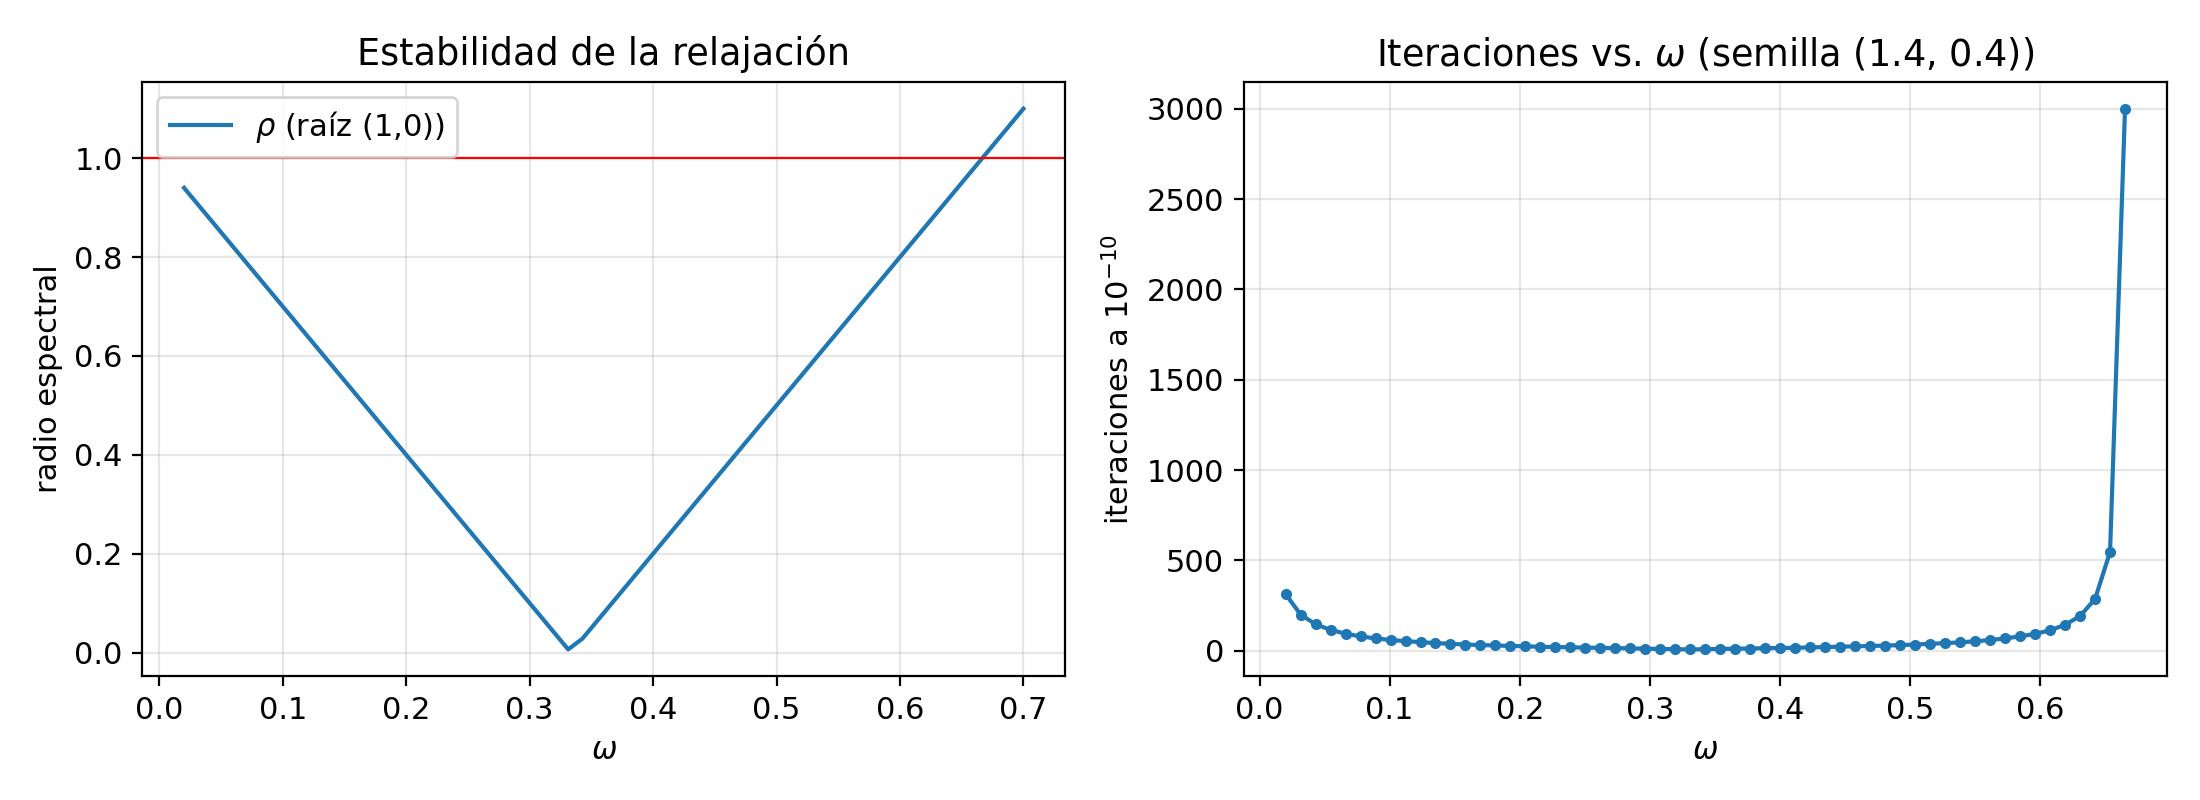
\includegraphics[width=.85\textwidth]{p4b_omega.png}
\caption{Radio espectral de la relajación (izquierda) e iteraciones necesarias (derecha) frente al parámetro de relajación $\omega$.}\label{fig:omega}
\end{figure}

\textbf{Método de Newton de dos variables.} Se linealiza $\vect F(\vect x)$: $\vect F(\vect x_k+\Delta\vect x)\approx\vect F(\vect x_k)+J(\vect x_k)\Delta\vect x=0$. En cada iteración se resuelve el sistema lineal
\begin{equation}
J(\vect x_k)\,\Delta\vect x=-\vect F(\vect x_k),\qquad \vect x_{k+1}=\vect x_k+\Delta\vect x, \label{eq:newton2d}
\end{equation}
con
\[
J=\begin{pmatrix}3x^2-3y^2&-6xy\\6xy&3x^2-3y^2\end{pmatrix}.
\]
La resolución de~\eqref{eq:newton2d} se hace en el programa con la misma función \texttt{gauss\_pivoteo} de la Unidad~1 (no hay ninguna llamada a un resolvedor externo): Newton multivariable reduce un problema no lineal a una sucesión de problemas lineales. La convergencia es cuadrática si $J$ es regular en la raíz, condición que se cumple porque $\det J=9|z|^4=9\neq0$ en las tres raíces. Para este sistema el error obedece $e_{k+1}\approx|1/z^*|\,e_k^2=e_k^2$.

\begin{table}[H]\centering\small
\resizebox{\textwidth}{!}{\begin{tabular}{r c c c c c}
\toprule
$k$ & $x_k$ & $y_k$ & $\|F(x_k)\|$ & $e_k$ & $e_{k+1}/e_k^2$\\
\midrule
0 & 1.400000000000 & 0.400000000000 & 2.53e+00 & 5.66e-01 & 0.611\\
1 & 1.066832799335 & 0.183600332265 & 6.30e-01 & 1.95e-01 & 0.897\\
2 & 0.979309412459 & 0.027308883073 & 1.01e-01 & 3.43e-02 & 1.028\\
3 & 0.999630446626 & -0.001148389261 & 3.62e-03 & 1.21e-03 & 1.000\\
4 & 0.999998815891 & 0.000000847387 & 4.37e-06 & 1.46e-06 & 1.000\\
5 & 1.000000000001 & -0.000000000002 & 6.36e-12 & 2.12e-12 & --\\
6 & 1.000000000000 & -0.000000000000 & 8.24e-24 & 2.75e-24 & --\\
7 & 1.000000000000 & 0.000000000000 & 0.00e+00 & 0.00e+00 & --\\
\bottomrule
\end{tabular}
}
\caption{Newton de dos variables desde $(1.4,\,0.4)$: $e_k$ es la distancia euclídea a la raíz $(1,0)$.}\label{tab:n2d}
\end{table}

Desde $(1.4,0.4)$ (Tabla~\ref{tab:n2d}) bastan 5 iteraciones para $\|\vect F\|\sim10^{-12}$ y 7 para el cero de máquina. El cociente $e_{k+1}/e_k^2$ va de $0.61$ a $1.000$ y confirma el valor teórico $1$, y $\|\vect F\|$ pasa de $2.5$ a $0.63$, $0.10$, $3.6\times10^{-3}$, $4.4\times10^{-6}$, $6.4\times10^{-12}$, $8.2\times10^{-24}$: los exponentes se duplican aproximadamente ($-3,-6,-12,-24$). En comparación, la relajación necesitó 30 iteraciones para $10^{-12}$: Newton es cuadrático y relajación lineal (Figura~\ref{fig:sis2d}, derecha). La Tabla~\ref{tab:n2do} recoge otras semillas: la solución alcanzada depende de dónde se empiece, y desde $(0.5,\,0.5)$ Newton no converge a la raíz más cercana a la semilla sino a $(-0.5,\,0.866)$ tras 10 iteraciones. Además, en el origen $J=0$ y la eliminación de Gauss detecta un pivote nulo (matriz singular) y lo señala con una excepción: es el punto donde Newton no está definido.

\begin{table}[H]\centering\small
\begin{tabular}{c c c c c}
\toprule
Caso & semilla $(x_0,y_0)$ & iteraciones & raíz alcanzada & $\|F\|$ final\\
\midrule
A & $(1.4,\,0.4)$ & 7 & $(1.0000,\,0.0000)$ & 0.0e+00\\
B & $(-0.3,\,0.6)$ & 7 & $(-0.5000,\,0.8660)$ & 2.5e-16\\
C & $(-0.3,\,-0.6)$ & 7 & $(-0.5000,\,-0.8660)$ & 2.5e-16\\
D & $(0.5,\,0.5)$ & 10 & $(-0.5000,\,0.8660)$ & 2.5e-16\\
\bottomrule
\end{tabular}

\caption{Newton de dos variables desde distintas semillas.}\label{tab:n2do}
\end{table}

\begin{figure}[H]\centering
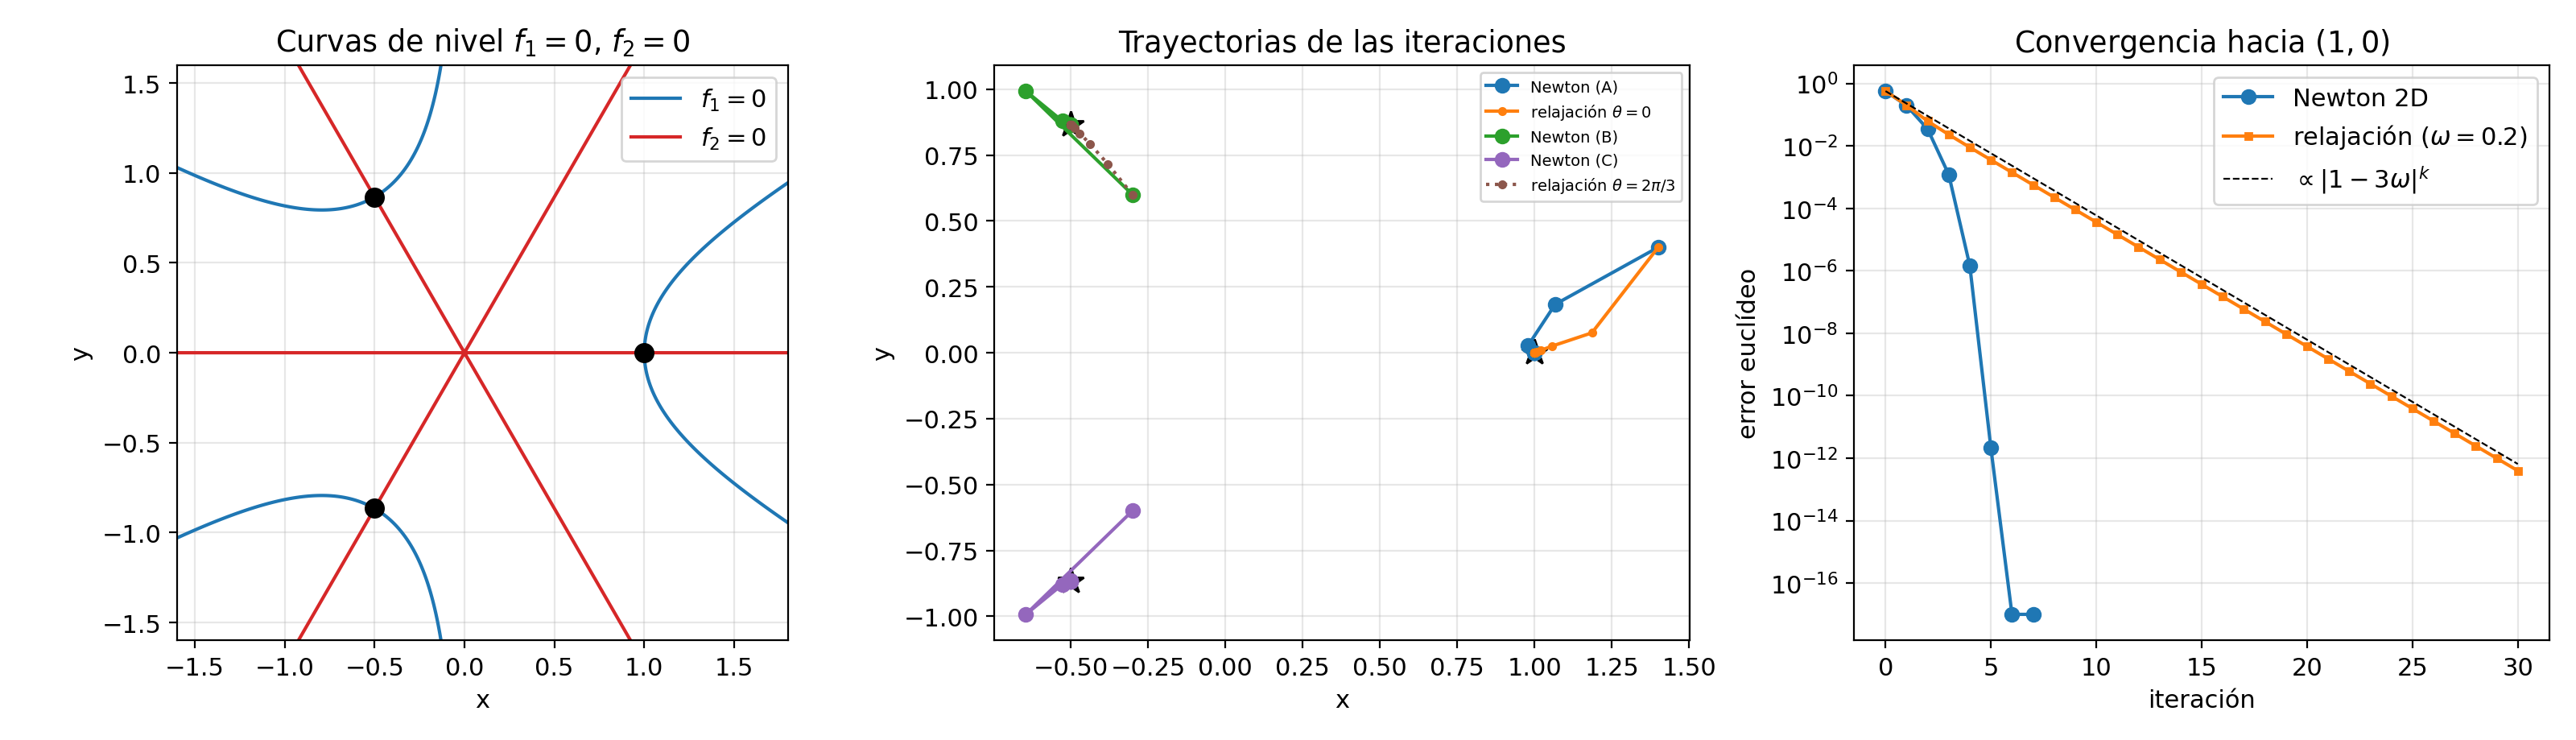
\includegraphics[width=\textwidth]{p4b_sistema.png}
\caption{Izquierda: curvas $f_1=0$ (azul) y $f_2=0$ (rojo) con las tres raíces. Centro: trayectorias de Newton y de la relajación en el plano $(x,y)$. Derecha: error frente a la iteración en escala semilogarítmica.}\label{fig:sis2d}
\end{figure}

La Figura~\ref{fig:cuencas} muestra las cuencas de atracción de Newton (cada color es la raíz alcanzada desde cada semilla; el cálculo usa la equivalencia $\vect x_{k+1}=\vect x_k-J^{-1}\vect F\Leftrightarrow z_{k+1}=z_k-(z_k^3-1)/(3z_k^2)$, válida porque $J$ es la multiplicación por $3z^2$). Las tres cuencas son regiones ramificadas cuya frontera es un fractal (conjunto de Julia): en el entorno de cada raíz Newton converge siempre, pero lejos de ellas pequeños cambios en la semilla producen resultados distintos. Esto responde por qué el método cuadrático es también el menos predecible en cuanto a \emph{qué} raíz encuentra, mientras que la relajación, más lenta, tiene un control explícito de su región de convergencia mediante $\omega$ y $\theta$.

\begin{figure}[H]\centering
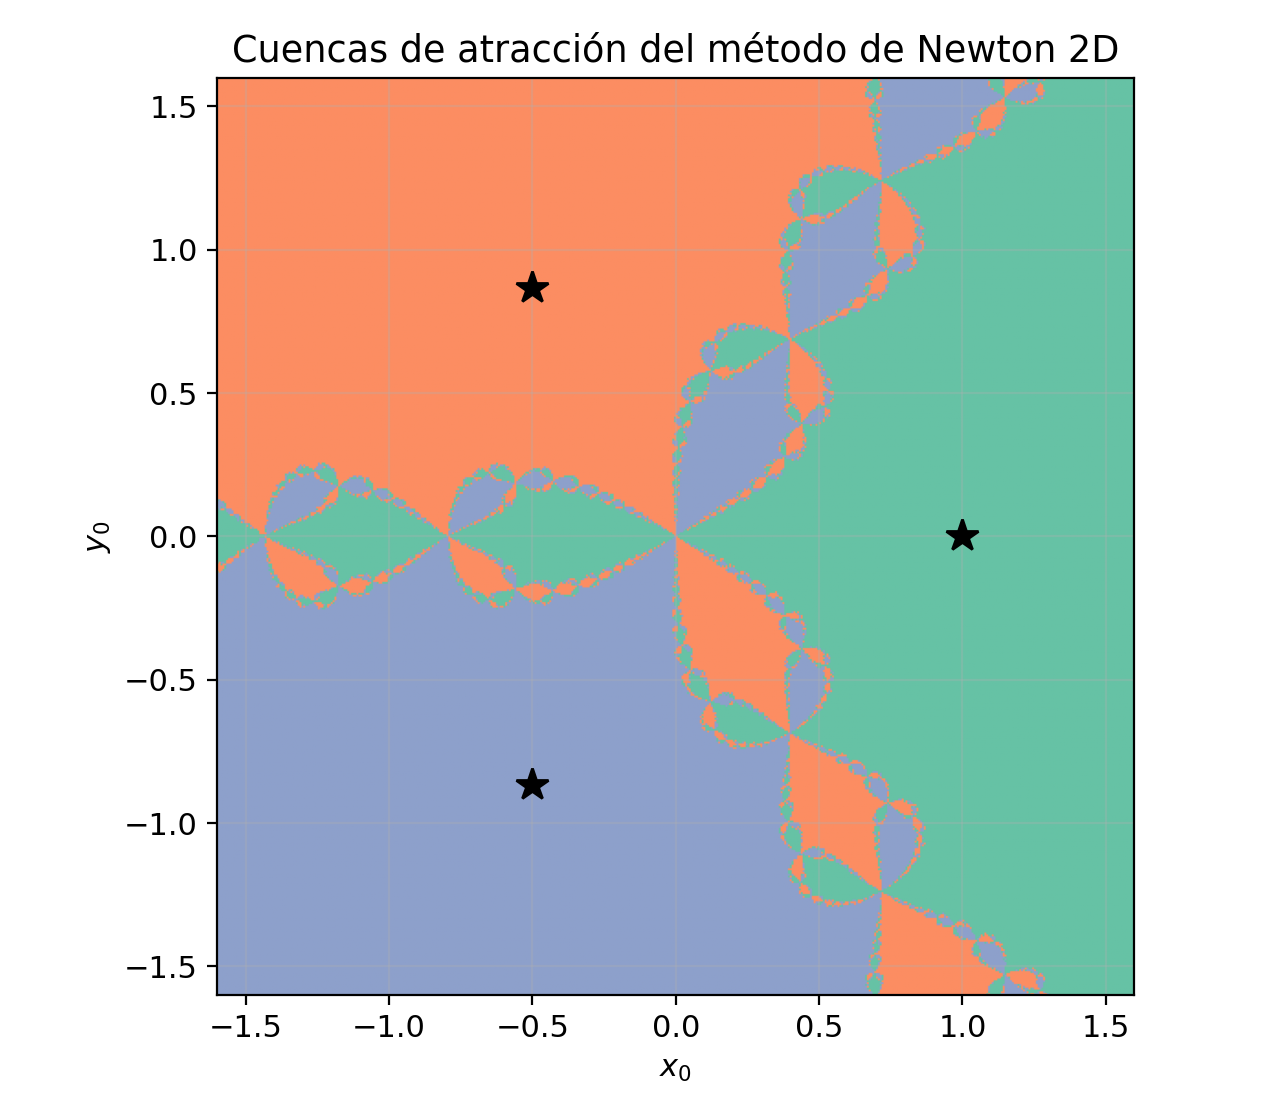
\includegraphics[width=.6\textwidth]{p4b_cuencas.png}
\caption{Cuencas de atracción de las tres raíces para el método de Newton de dos variables.}\label{fig:cuencas}
\end{figure}

%=====================================================================
\section{Conclusiones}
%=====================================================================
En el \textbf{Problema~1} se verificó que la barra con fuente uniforme o cúbica se resuelve de forma exacta en los nodos (error de redondeo, $\sim10^{-14}$ ºC) y con error $O(\Delta x^2)$ cuando la solución contiene un seno, con un orden observado de $1.98$--$2.00$. La eliminación de Gauss y la factorización de Thomas dan resultados idénticos, pero Thomas cuesta $O(N)$ y permite cambiar la fuente sin refactorizar; el pivoteo parcial no se necesita en esta matriz, pero es indispensable en general (demostración con $\varepsilon=10^{-17}$). La inversa, con fórmula cerrada $\min(i,j)(N+1-\max(i,j))/(N+1)$, es la función de Green discreta: contiene toda la respuesta lineal del sistema.

En el \textbf{Problema~2} los cuatro modos tienen frecuencias $12.36$, $23.51$, $32.36$ y $38.04$ rad/s ($1.97$--$6.05$ Hz), con perfiles sinusoidales de $j-1$ nodos. Jacobi (cuatro barridos, convergencia cuadrática) y potencia con deflación coinciden con la solución analítica $\omega_j=40\sin(j\pi/10)$; Jacobi es más preciso porque no arrastra error por la deflación.

En el \textbf{Problema~3} la relajación converge siempre para $e<1$ porque $|g'|\le e$, con velocidad $\rho=e|\cos E^*|$: 3 iteraciones para $e=0.1$ y 24 para $e=0.92$. La bisección necesita 23 iteraciones para cualquier $e$. La relajación gana mientras $\rho<1/2$, y esa condición se pierde antes en las anomalías medias pequeñas ($e\gtrsim0.63$ con $M=0.1$, $e\gtrsim0.91$ con $M=1.5$).

En el \textbf{Problema~4} el volumen molar del CO$_2$ es $v^*=1.13545\times10^{-3}$ m$^3$/mol ($Z=0.910$). Newton muestra orden $2.000$ con constante $126.997$, igual a la teórica $f''/2f'$, y la secante orden $\approx1.62$; el índice de eficiencia favorece a la secante ($1.618$ frente a $1.414$). En el sistema $z^3=1$, la relajación tiene convergencia lineal con la razón espectral predicha ($0.4$) y requiere ajustar $\omega$ y el giro $\theta$ para cada raíz, mientras que Newton multivariable, con la eliminación de Gauss de la Unidad~1 en cada paso, alcanza la precisión de máquina en 7 iteraciones, a costa de una dependencia fractal de la semilla y de la posible singularidad de $J$.

\appendix
\section{Código del módulo \texttt{metodos.py}}
Los programas \texttt{problema1.py}--\texttt{problema4.py} (entregados junto a este informe) construyen los sistemas de cada problema, llaman a estas funciones y generan las tablas y figuras. Para reproducirlo basta ejecutar \texttt{python3 problema1.py}, \dots, \texttt{python3 problema4.py} en la carpeta que contiene \texttt{metodos.py}.
\lstinputlisting{metodos.py}

\end{document}
